\chapter{Robot bicycle}

\section{Introduction and Motivation} \label{rb:sec:intro}

The Whipple bicycle model qualitatively predicts behavior commonly observed in
physical bicycles such as a stable speed range and counter steer. To
quantitatively assess the accuracy of these predictions, in as controlled a
setting as possible, a robot bicycle was constructed. By \textit{robot
bicycle}, we simply mean a bicycle that can balance without a human rider; this key
feature permits experiments to be performed where dynamic quantities can be
measured without the influence of undesirable and difficult to measure human
inputs such as limb motion. Measurement of the bicycle motion that results from
the application of precisely known bicycle inputs permits direct comparisons to
predictions of the Whipple model without the need to model the human.
Experiments such as those conducted by Kooijman~\cite{Kooijman2007}, wherein a
riderless bicycle was pushed and ``ghost ridden'', do not maintain a constant
speed (the bicycle decelerates as soon as it is released by the pusher), nor
can a specific initial speed be set easily or precisely. Additionally,
in~\cite{Kooijman2007}, only the uncontrolled bicycle dynamics were examined;
as such, it was limited to speeds for which the uncontrolled bicycle is stable.
This work extends the work of~\cite{Kooijman2007} by accurately maintaining a
constant speed, and stabilizing the bicycle for speeds below the weave speed.

% TODO: motivate more discuss system identification
% if you remove the rider, the bicycle has a single input
% talk about system id
% bicycle is unstable
% control must be based upon some model of the bicycle
% for some frequencies, the model is sufficient (low bandwidth control
% for others it is not (high frequencies not predicted by the model)

This chapter describes the design and construction (mechanical, electrical, and
software) of the robot bicycle and presents data collected in a set of experiments.
Physical parameter measurement, sensor calibration, and all mechanical and
electrical components (purchased and fabricated) are documented here. The
mechanical and electrical sections are somewhat low level and tedious but are
included for completeness. Readers interested in the high level control system
design may consider skipping to \autoref{rb:sec:control}. Finally, a
description and analysis of a set of experiments is presented.

\section{Mechanical construction} \label{rb:sec:mec}
\subsection{Design} \label{rb:subsec:mecdesign}
The robot bicycle is shown in Figures
\ref{rb:img:rightside}-\ref{rb:img:leftsidecloseup}. Where possible, readily
available bicycle parts were used. A number of components were fabricated to
interface standard bicycle parts (frame, fork steer tube, disc brake tabs) with
equipment not typically found on a bicycle (batteries, fork motor, safety
casters, and electrical equipment). This section provides a high level overview
of the construction; more details of each subsystem can be found in the
subsequent subsections pertaining to each piece of equipment.

\begin{figure}[ht]
  \centering
  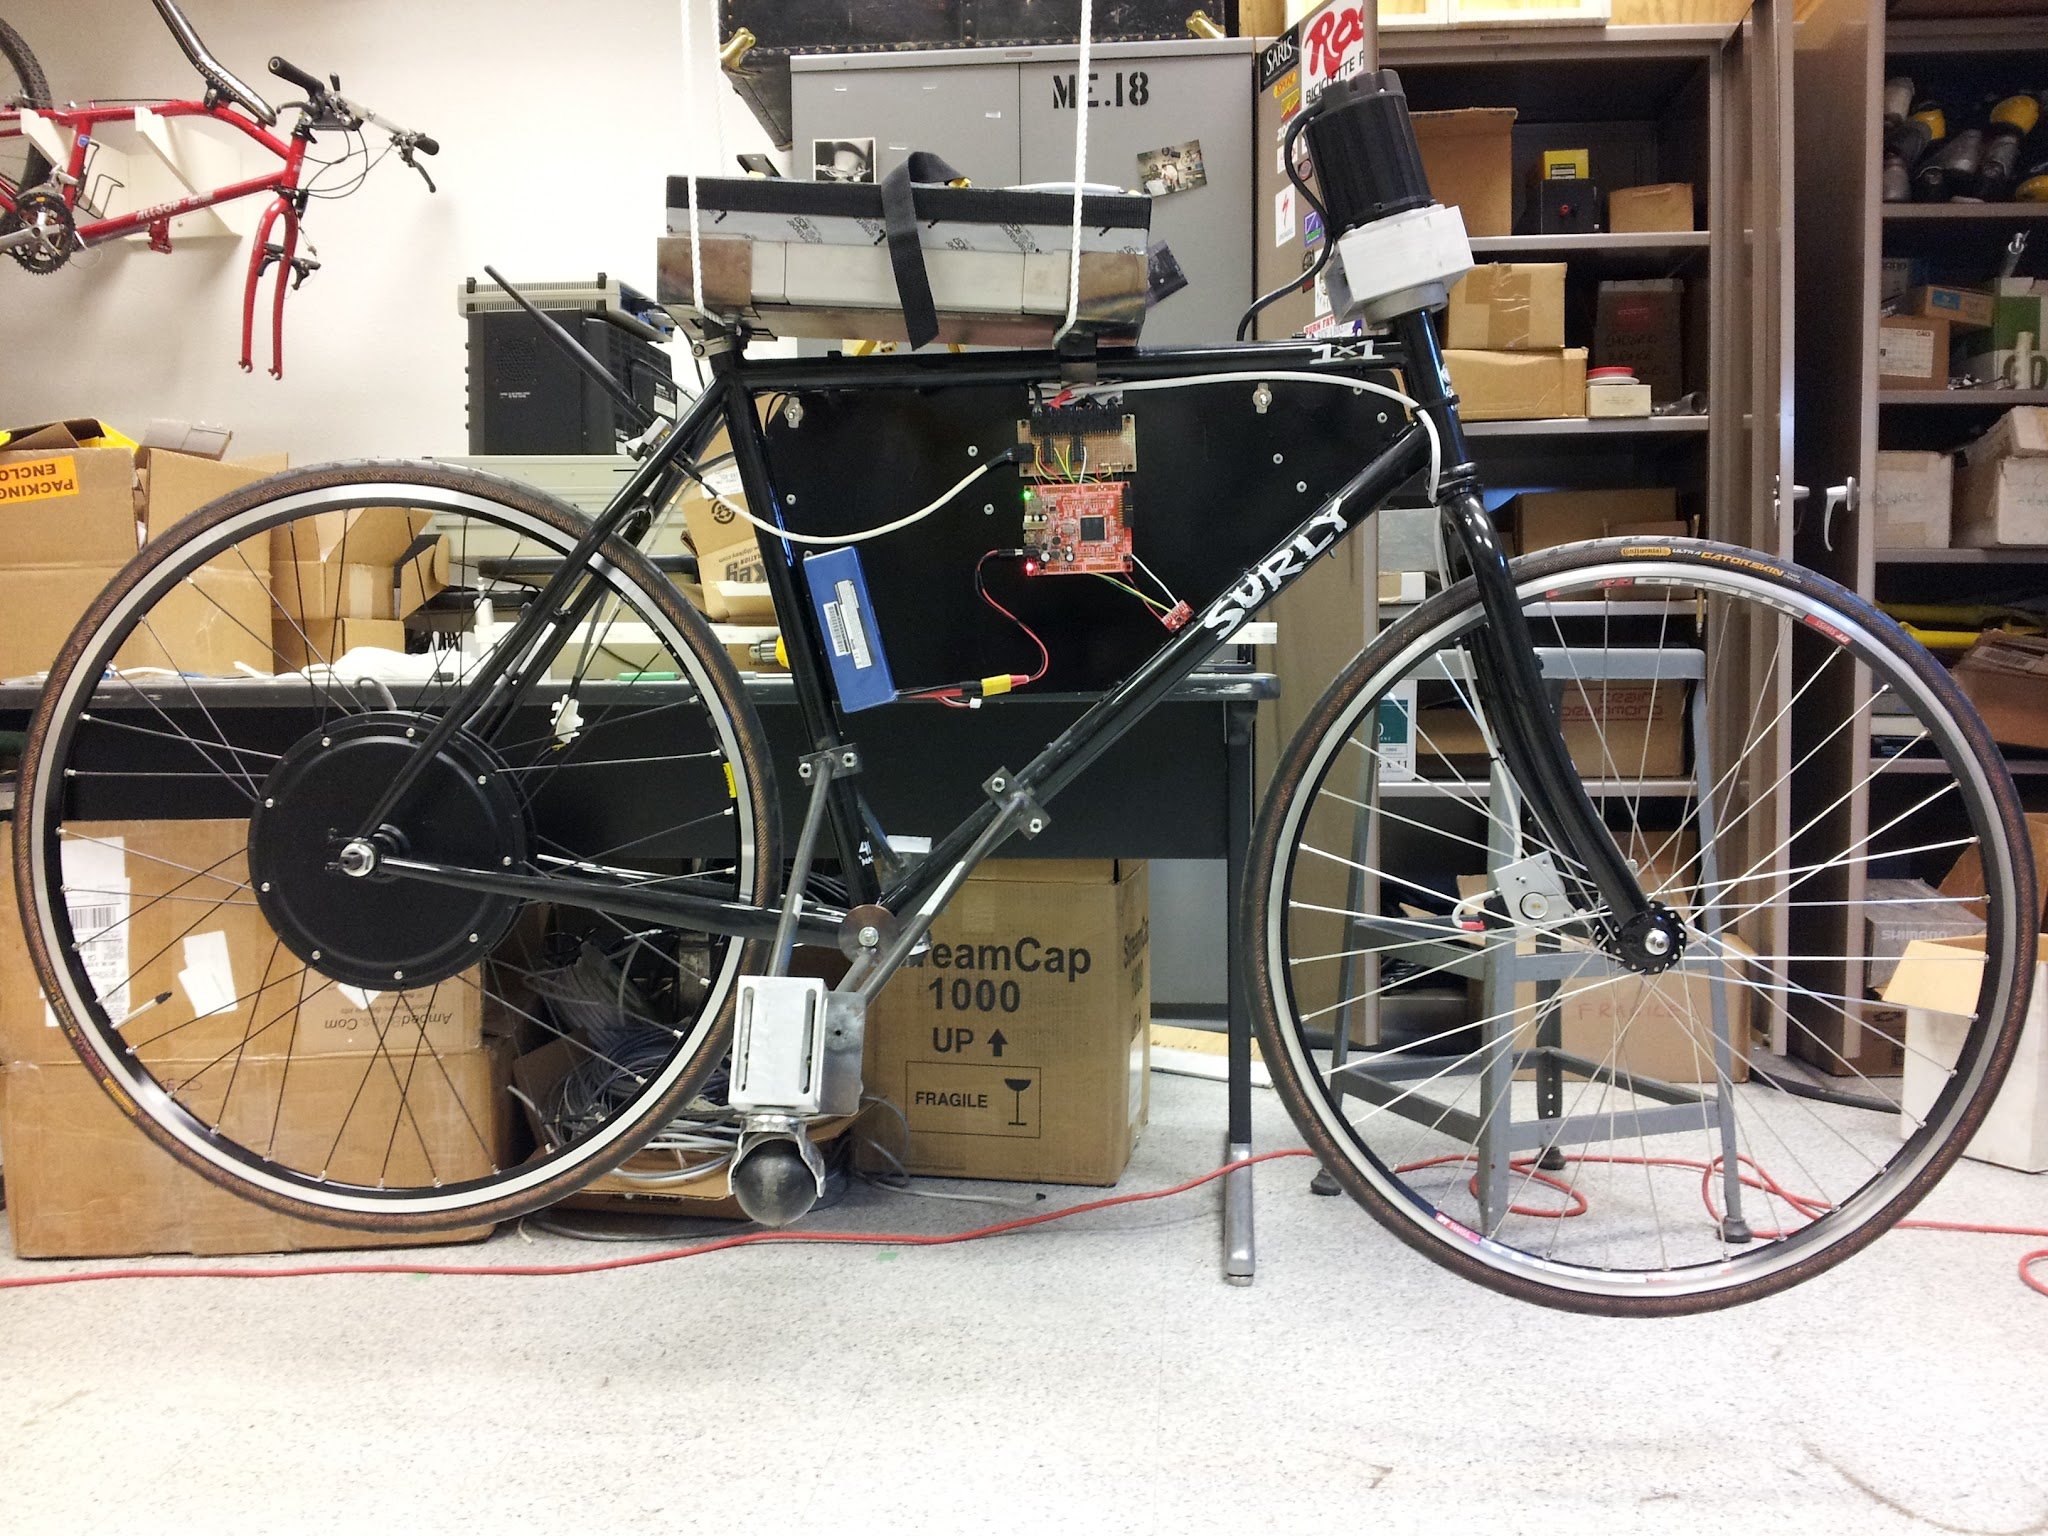
\includegraphics[width=\textwidth]{images/IMG_20120928_153020.jpg}
  \caption{Robot bicycle viewed from the right side.}
  \label{rb:img:rightside}
\end{figure}
\begin{figure}[h]
  \centering
  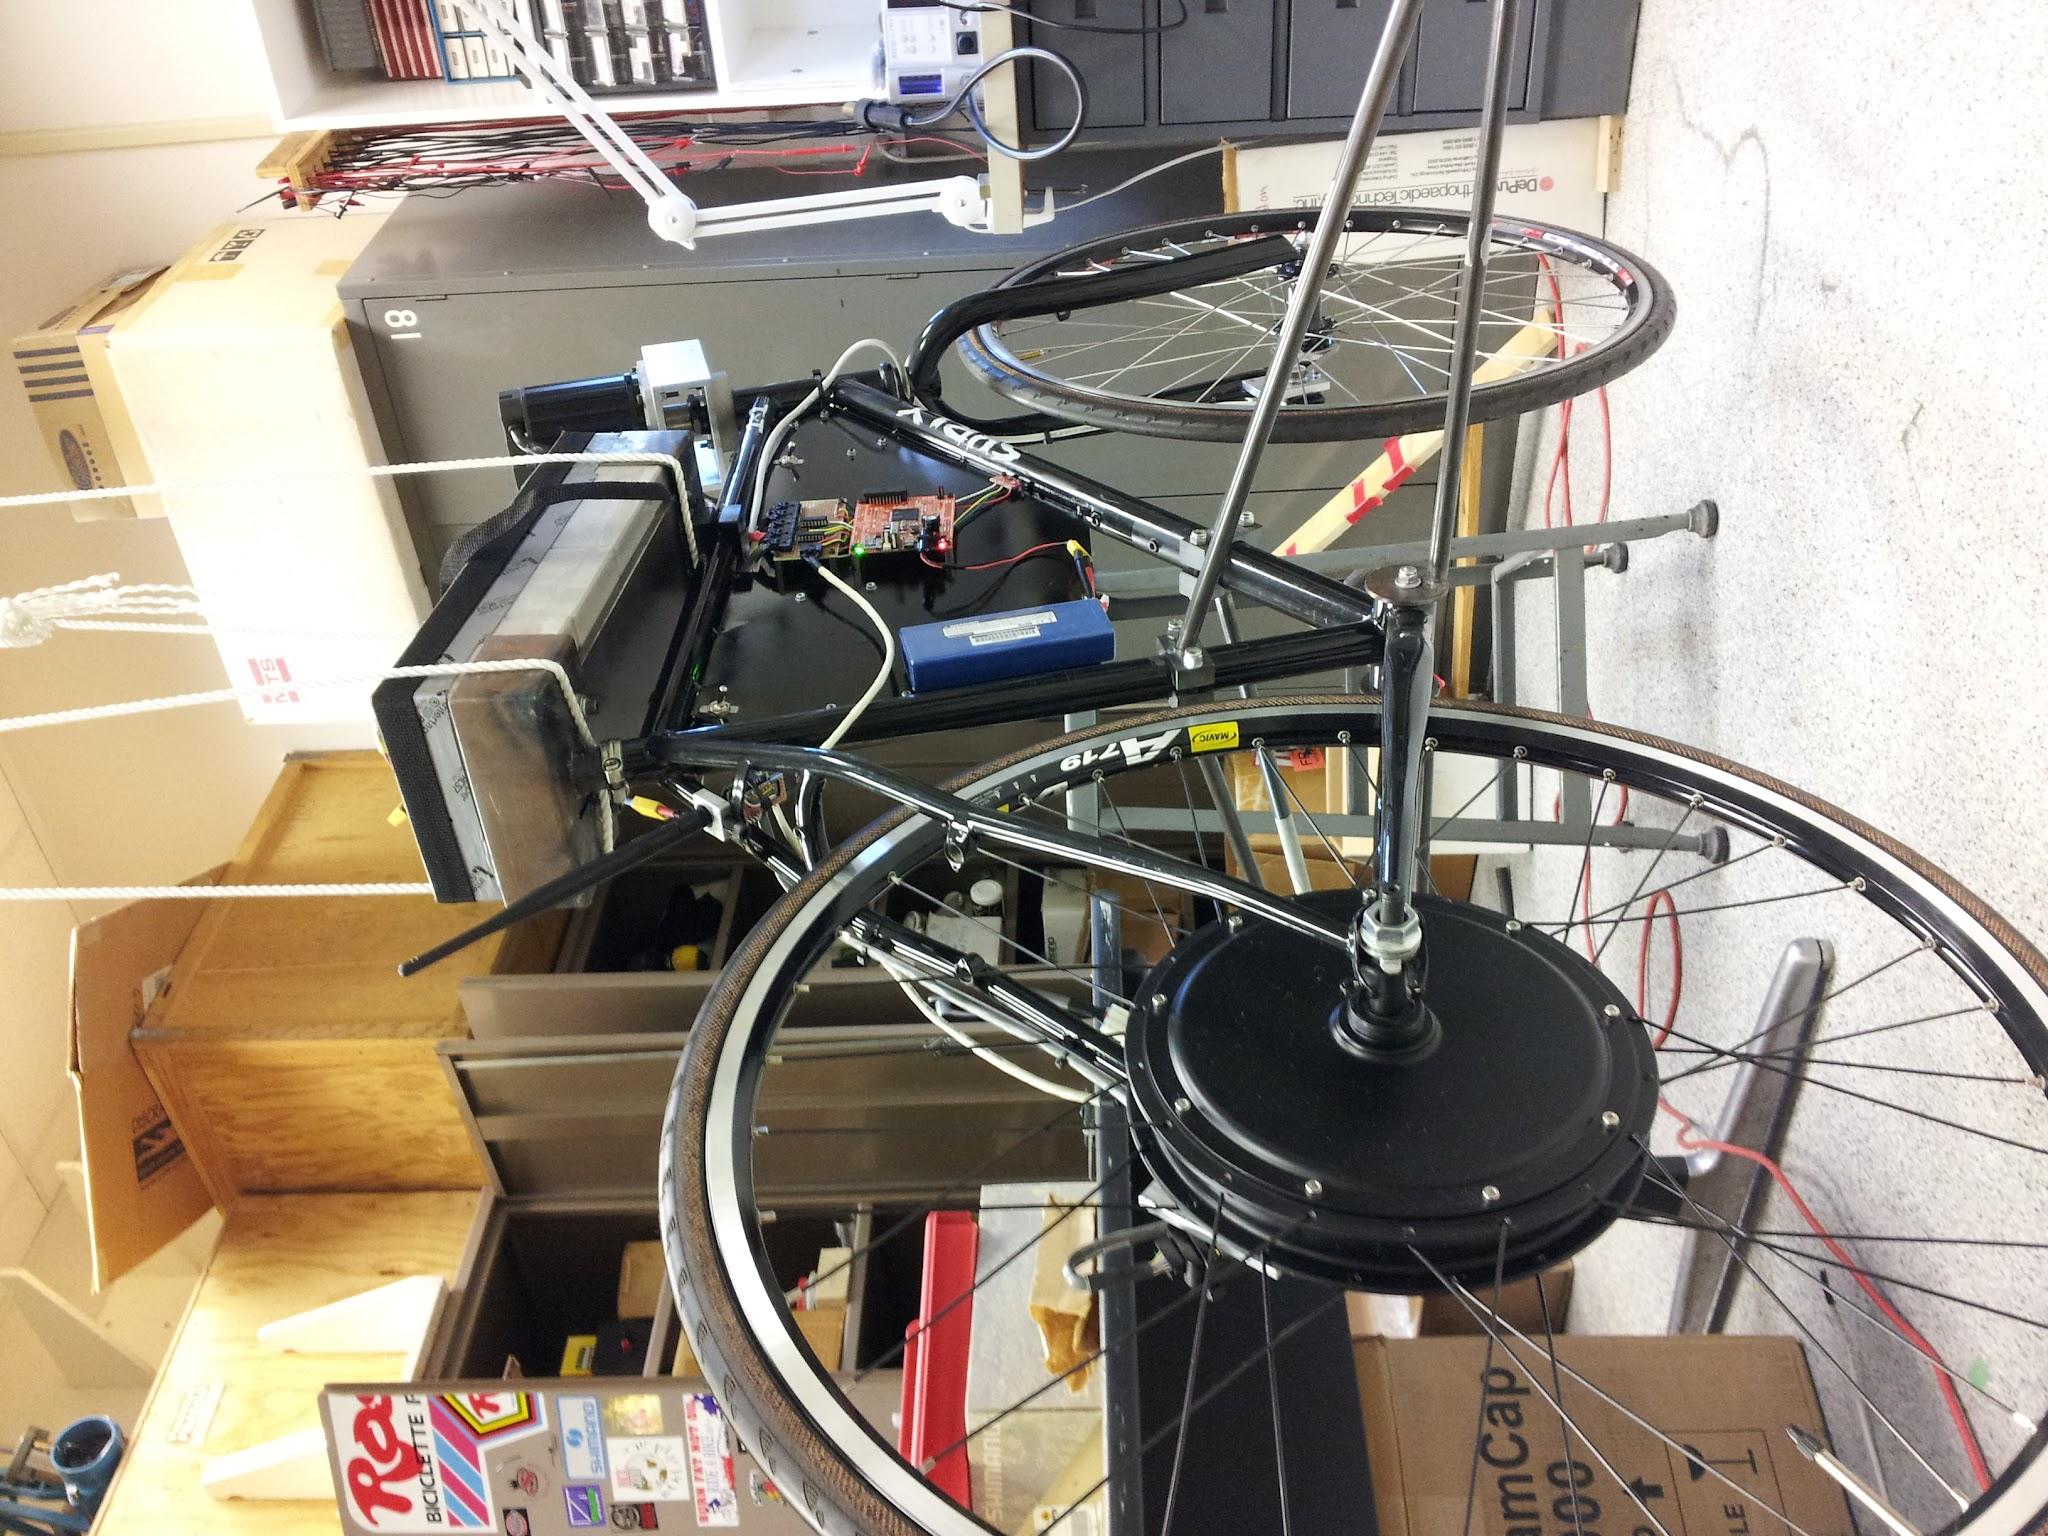
\includegraphics[width=\textwidth,angle=-90]{images/IMG_20120928_153146.jpg}
  \caption{Robot bicycle viewed from the rear right side. The wireless antenna
  is visible behind the batteries, and the attachment of the training wheel
struts to the bicycle frame can also be seen.}
  \label{rb:img:rearrightside}
\end{figure}
\begin{figure}[h]
  \centering
  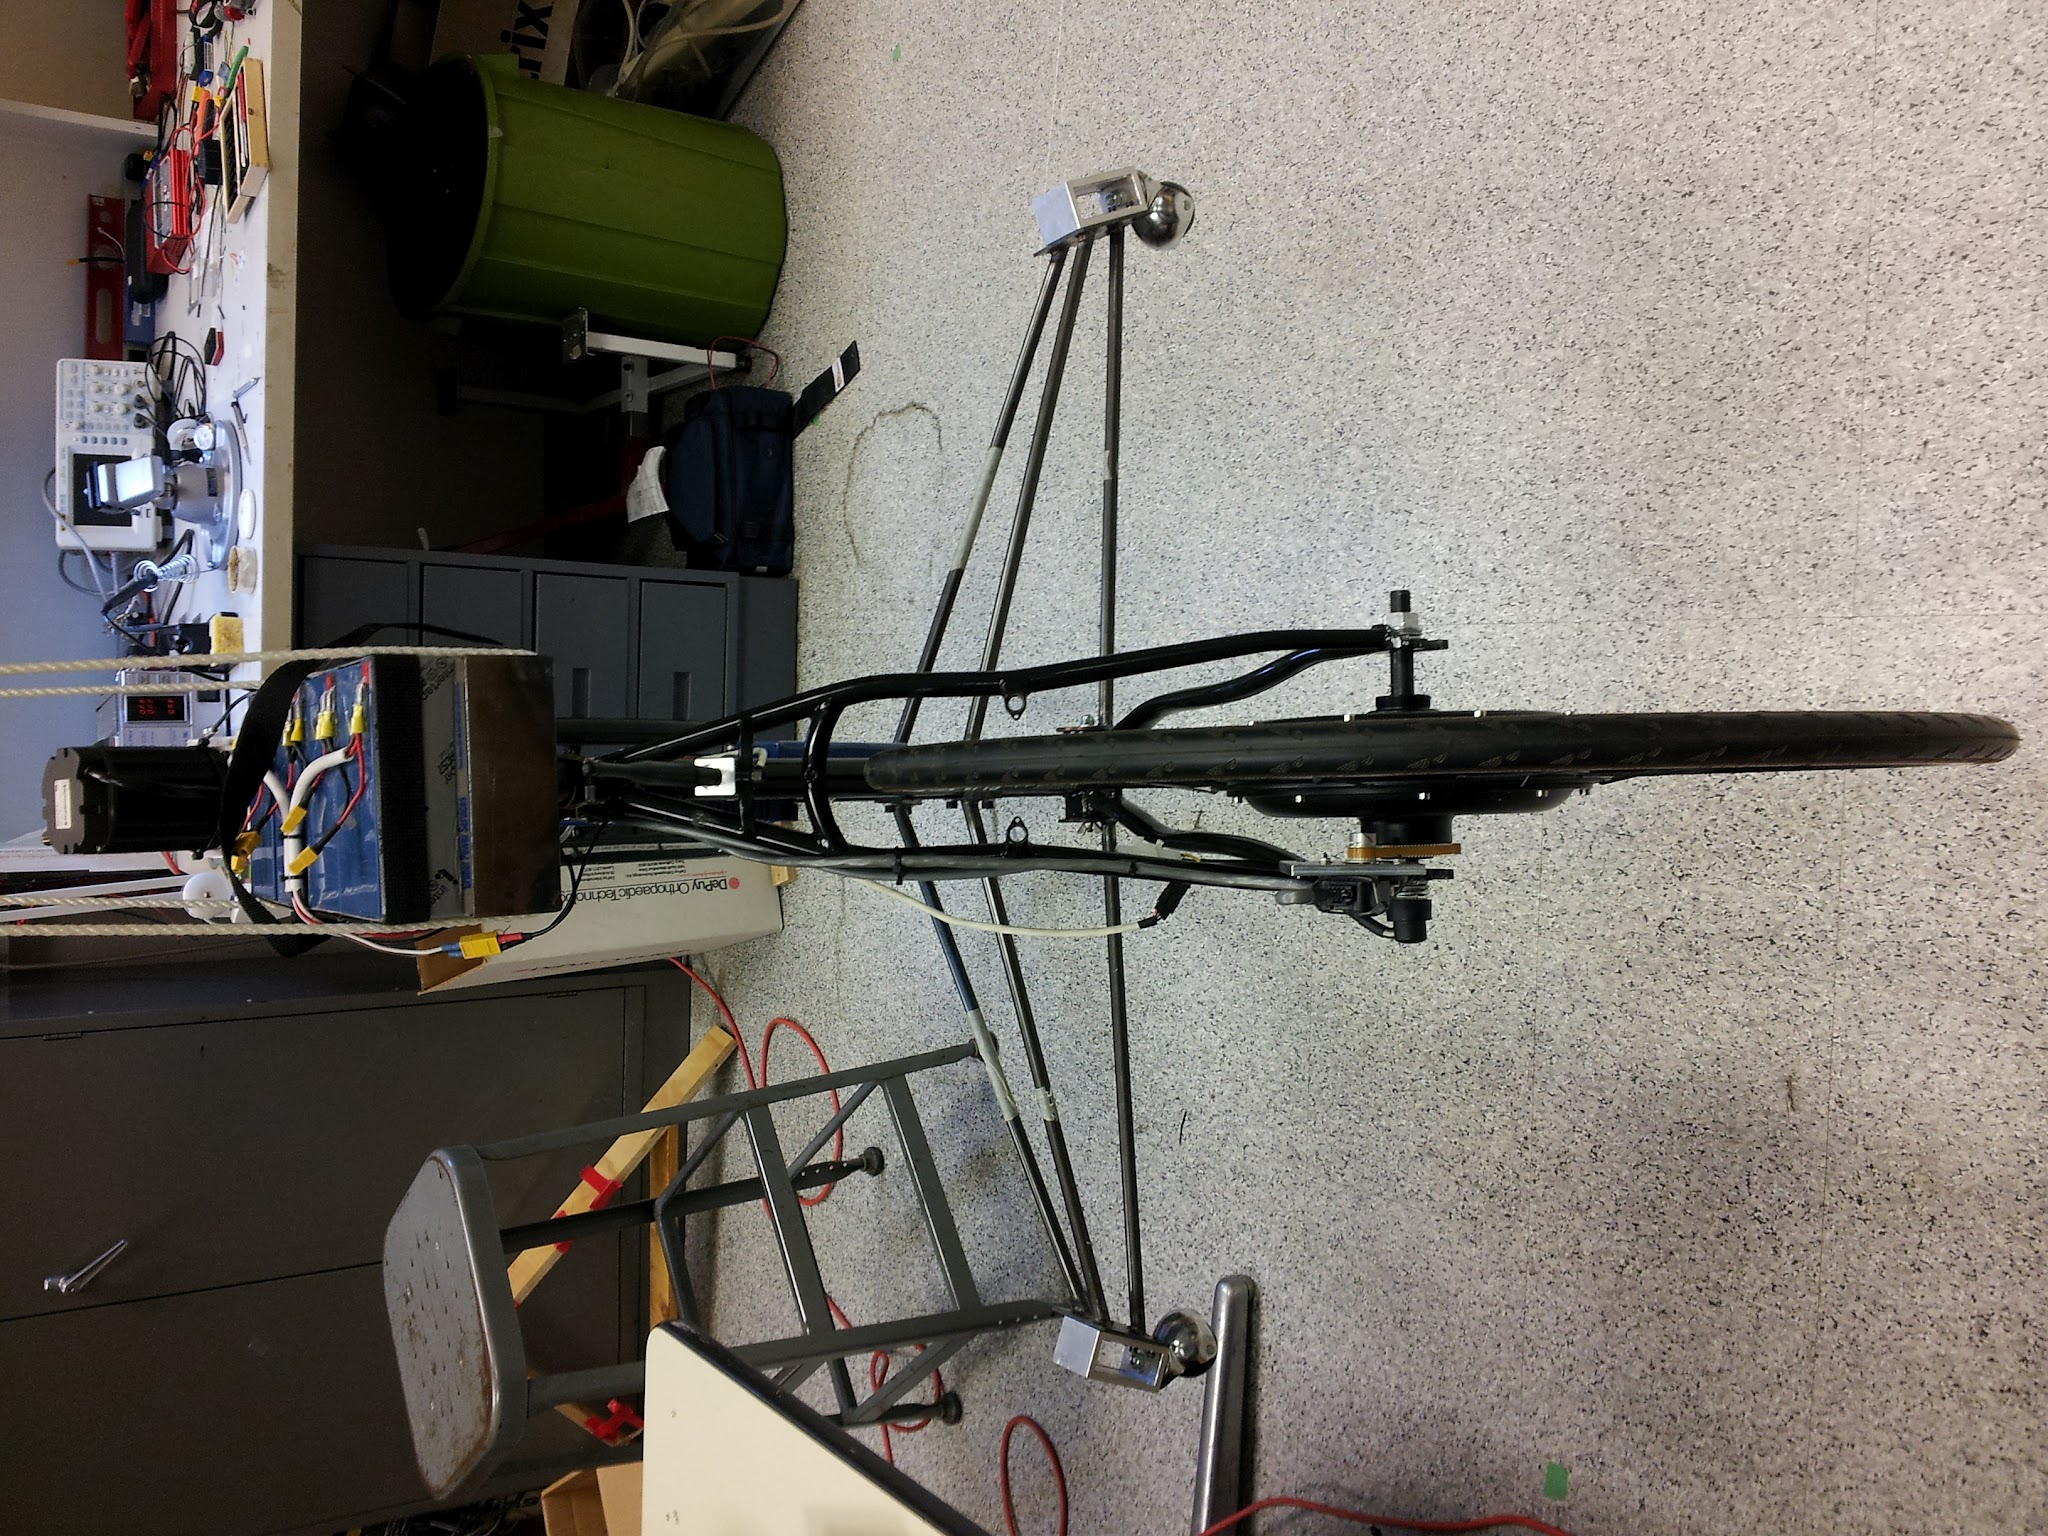
\includegraphics[width=\textwidth,angle=-90]{images/IMG_20120928_153405.jpg}
  \caption{Robot bicycle viewed from the rear.}
  \label{rb:img:rear}
\end{figure}
\begin{figure}[h]
  \centering
  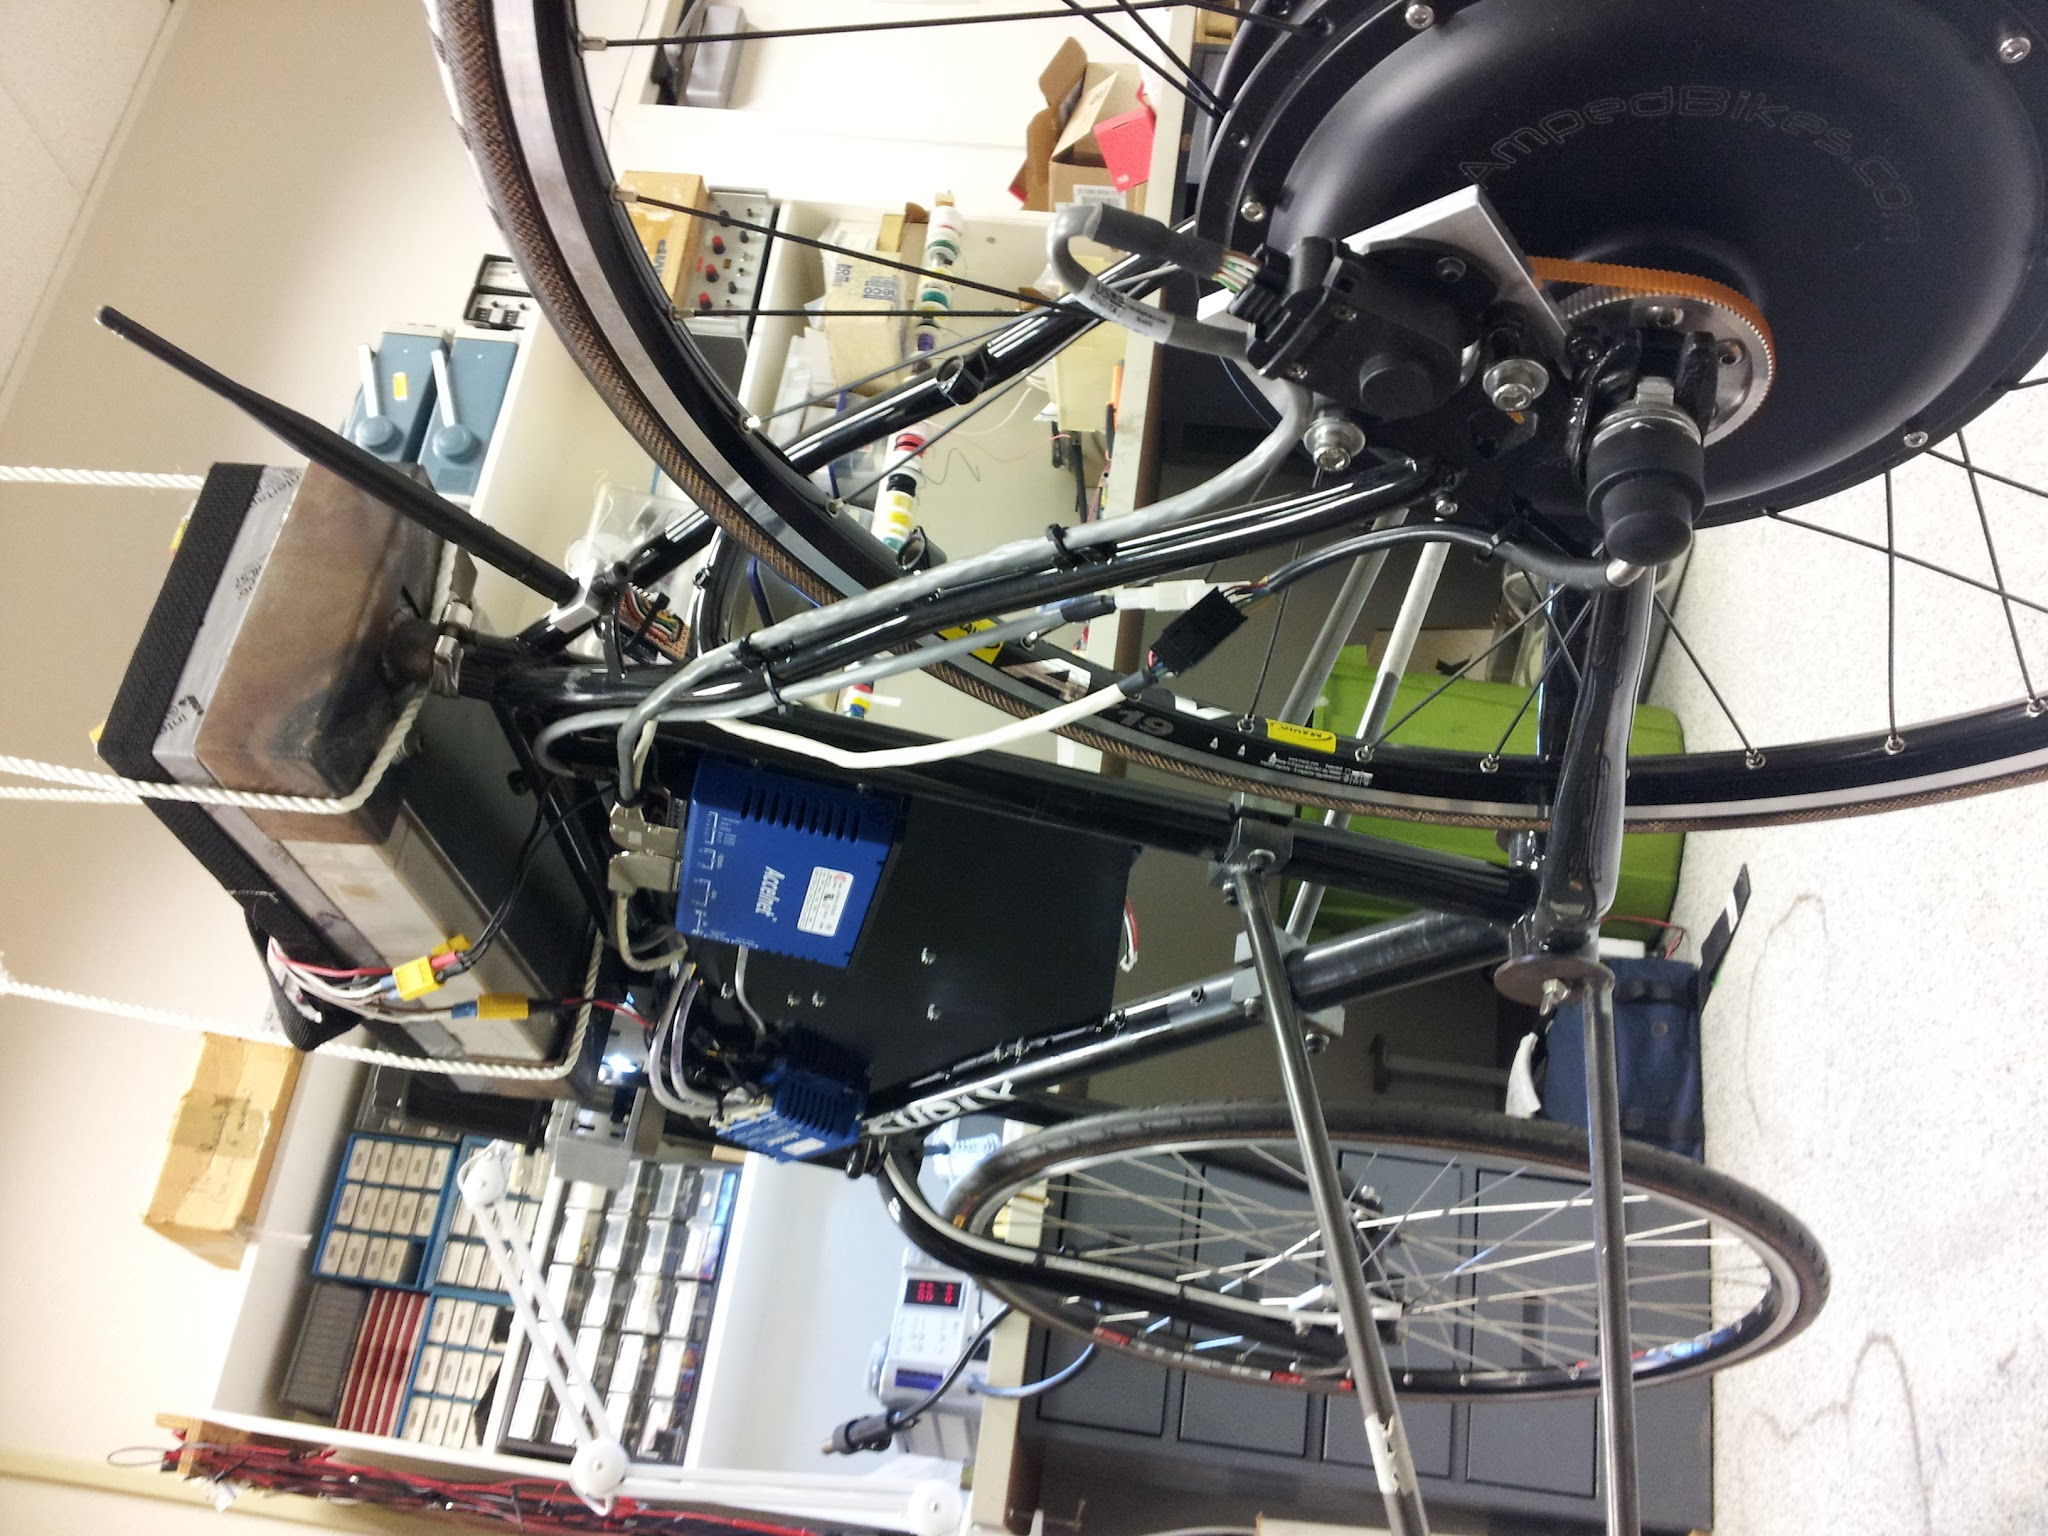
\includegraphics[width=\textwidth,angle=-90]{images/IMG_20120928_153321.jpg}
  \caption{Robot bicycle viewed from the rear left. The motor wiring exits the
    left side of the rear wheel axle. The rear wheel optical encoder is mounted
    to the rear disc brake tabs and is driven by the rear wheel with a
    toothed kevlar belt combined with 100 tooth and 25 tooth pulleys.}
  \label{rb:img:rearleftside}
\end{figure}
\begin{figure}[h]
  \centering
  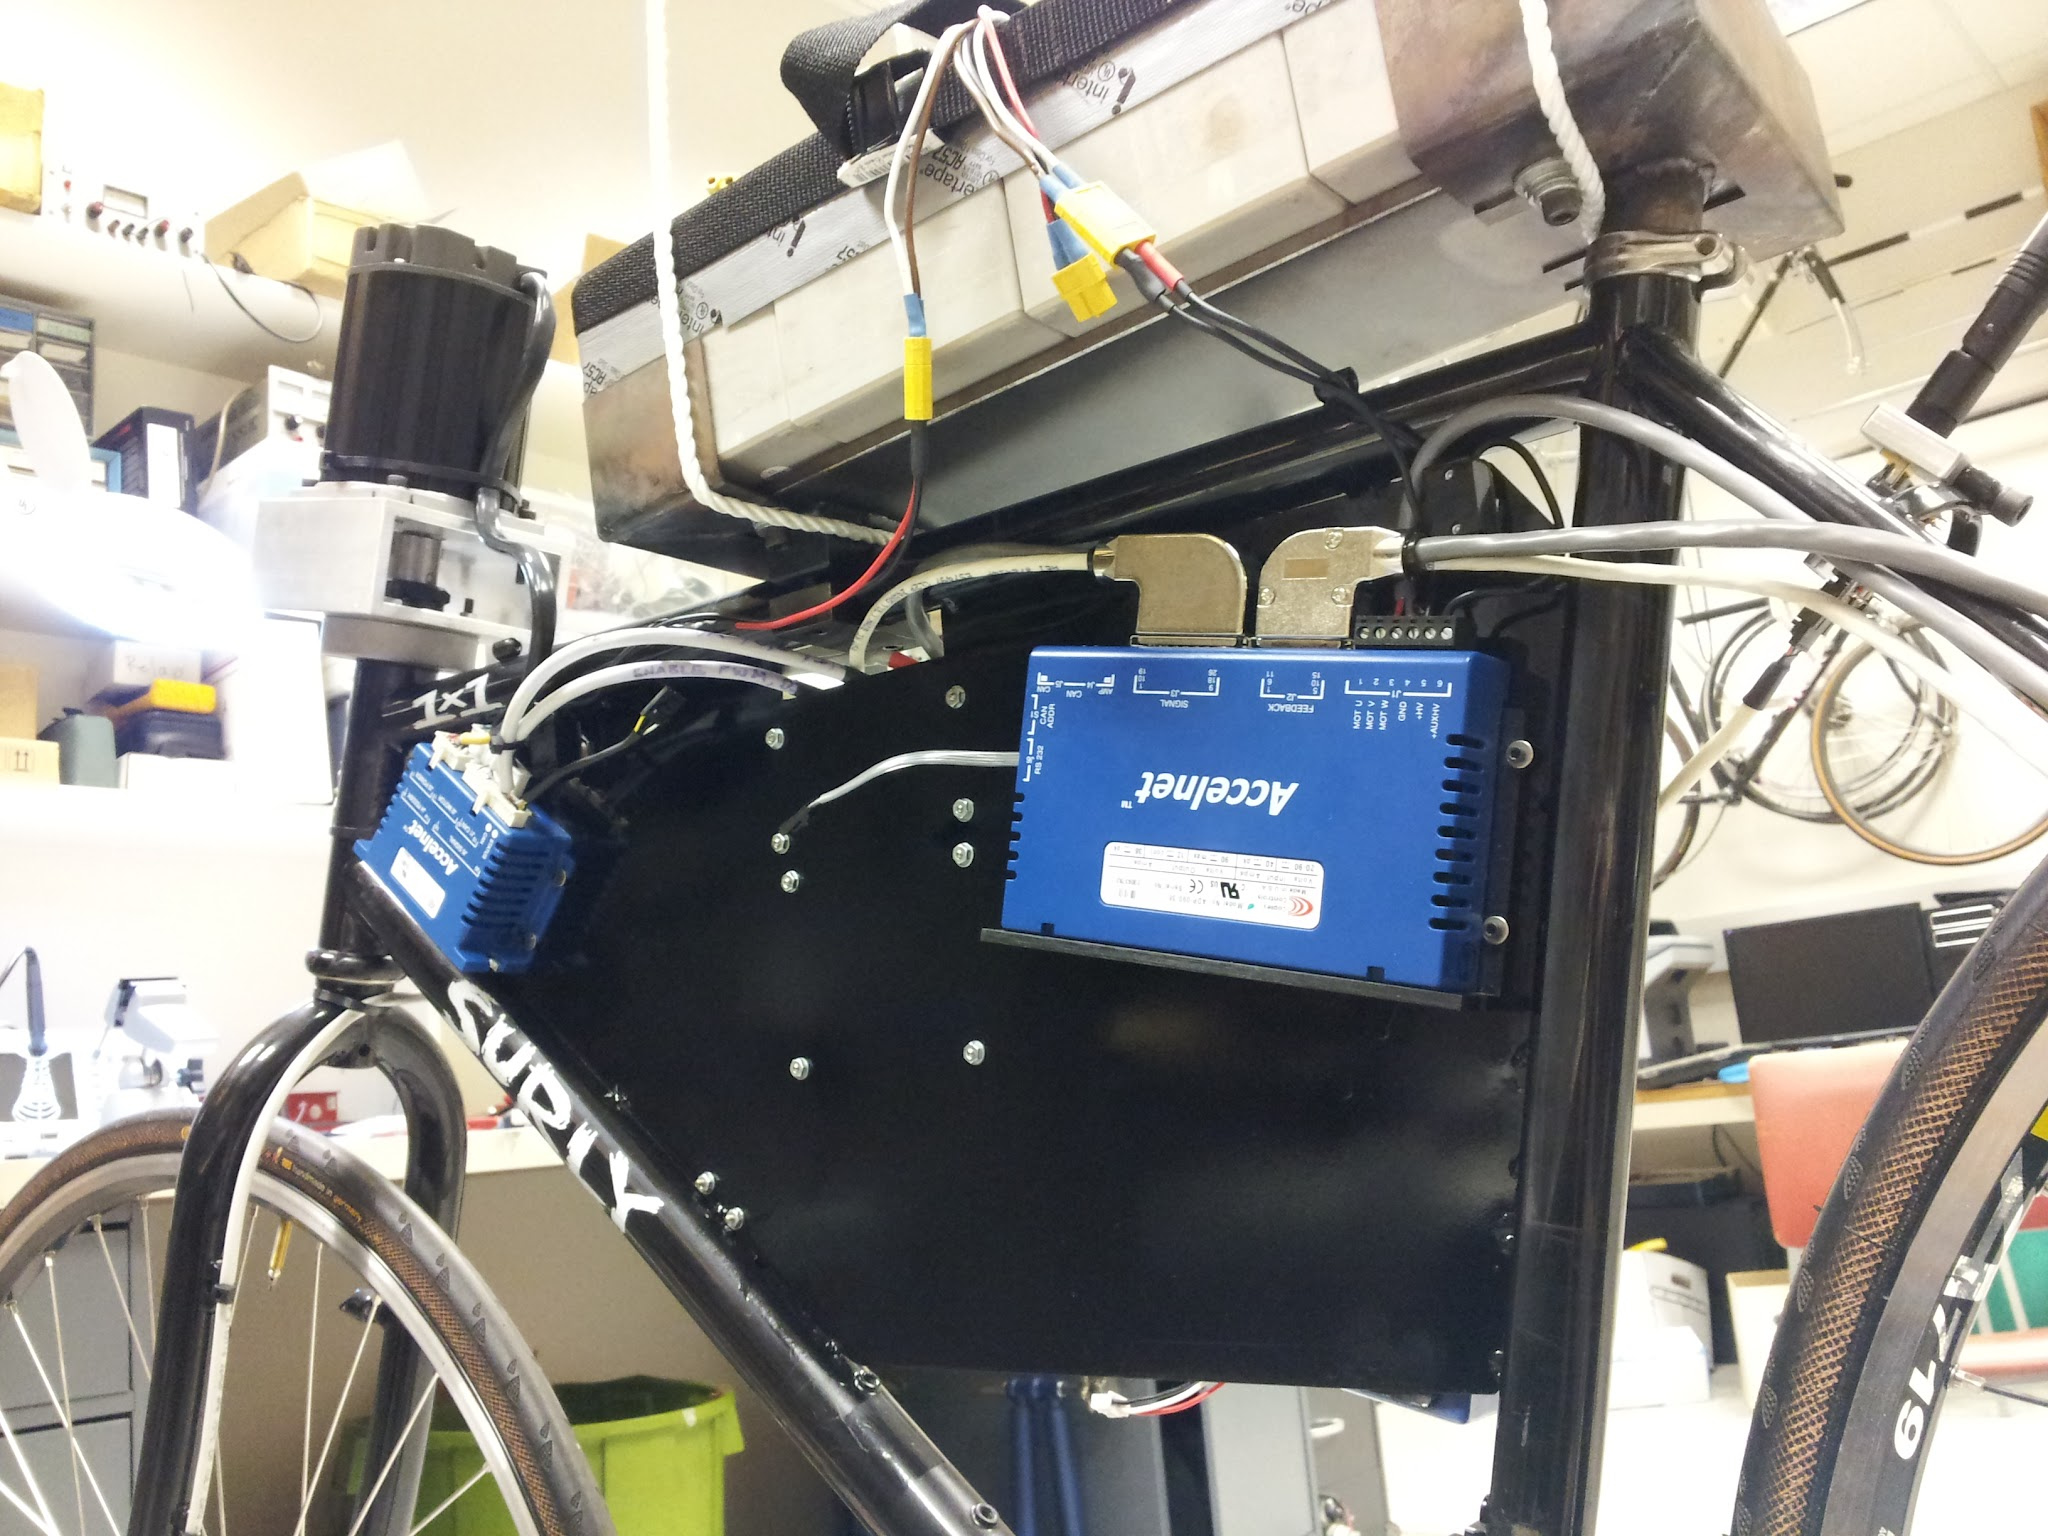
\includegraphics[width=\textwidth]{images/IMG_20120928_153336.jpg}
  \caption{Close up of battery plate, fork motor mount, and digital motor
  drives. The cylindrical plug interfacing the fork motor spindle and the fork
steer tube is visible inside the aluminum box section directly beneath the
steer motor.}
  \label{rb:img:leftsidecloseup}
\end{figure}

A Surly 4130 cromoly steel bicycle frame and fork were used~\cite{Surly2009}.
The frame and fork permit the use of 26'' or 700c wheels, cantilever or disc
brakes, and were chosen because its rugged steel construction permitted
modification without fear of compromising its structural integrity. The frame
was modified by welding an 18 gauge mild steel sheet to the inside of the front
triangle to provide a surface on which to mount the digital motor drives,
microcontroller development board and batteries.

To prevent damage to the robot bicycle in the case of a fall, custom training
wheels were designed and built. The training wheels were composed of casters
positioned approximately 18'' from the frame plane and roughly even with the
bottom bracket. The height of the casters permitted the bicycle to lean
approximately 20$^{\circ}$ before they touched the ground. Each caster wheel
was bolted to a 2'' long 2''x4'' aluminum box section which was in turn bolted
to one side of a small vertical steel plate. On the other side of the steel
plate, three 1/2''x0.0625'' 4130 cromoly steel round tubes were welded -- each
tube connected the steel plate (and hence the casters) to the bicycle frame and
provided sufficient strength and rigidity to handle the loads transmitted
during a fall. Welded to the inboard ends of the three 1/2'' tubes were
brackets which interfaced with the seat tube, down tube, and bottom bracket. The
brackets on either side of the frame were bolted together, thereby sandwiching
the bicycle frame.

Other custom-fabricated mechanical components were the wheel optical encoder
mounts, fork motor mounting hardware, and battery support plate. The details of
each of these components are discussed in \ref{rb:subsec:sensors},
\ref{rb:subsec:actuators}, and \ref{rb:subsec:batteries}, respectively.

\subsection{Physical parameter measurement} \label{rb:subsec:parameters}
The twenty three physical parameters (described in \autoref{chapter2}) of the
robot bicycle were estimated by measuring first the benchmark parameter set,
and then converting those parameters to the gyrostat parameter set using the
equations presented in \autoref{model:parameter_conversion}. It was assumed
that the wheel minor radius was zero (i.e., that the wheels were knife edged).
The resulting parameters are presented in \autoref{rb:tab:parameters}.

\begin{table}[ht]
  \centering
  \begin{tabular}{rccl}
    \toprule
    & {Rear gyrostat} & {Front gyrostat} & {Units} \\
    \midrule
    $I_{xx}$ &  1.542 &   0.183 & \si{kg.m^2} \\
    $I_{yy}$ &  3.557 &   0.226 & \si{kg.m^2} \\
    $I_{zz}$ &  3.014 &   0.069 & \si{kg.m^2} \\
    $I_{xz}$ &  0.839 &  -0.010 & \si{kg.m^2} \\
         $J$ &  0.114 &   0.092 & \si{kg.m^2} \\
         $m$ & 34.1   &   2.95  & \si{kg}     \\
         $R$ &  0.336 &   0.336 & \si{m}      \\
         $r$ &  0     &   0     & \si{m}\\
         $a$ &  0.514 &  -0.021 & \si{m}\\
         $b$ & -0.219 &  -0.152 & \si{m}\\
         $c$ &  0.963 &  -0.048 & \si{m}\\
         $l_s$ & \multicolumn{2}{c}{0.343} &  \si{m} \\
    \bottomrule
  \end{tabular}
  \caption{Robot bicycle physical parameters.}
  \label{rb:tab:parameters}
\end{table}

\section{Electrical system description} \label{rb:sec:elec}
\subsection{Microcontroller} \label{rb:subsec:mcu} All functionality related to
control, measurement, and user interaction was implemented by programming an
Olimex STM32-H407~\cite{OlimexSTM32H407} development board. A summary of the
board functionality utilized are shown in Table \ref{rb:tab:mcu}.
\begin{table}[h]
  \centering
  \begin{tabular}{|l|l|}
    \hline
        & ST Microelectronics STM32F407ZGT6 @ 168MHz \\
    CPU & 1MiB flash memory, 192KiB ram, 32-bit memory address space \\
        & Thumb-2 instruction set, single precision floating point \\
    \hline
           & 3 x 16-bit timers in quadrature counting mode \\
    Timers & 32-bit count up timer @ 4MHz \\
           & PWM generation @ 2.563KHz; $2^{16} - 1$ distinct duty cycles \\
    \hline
                   & UART peripheral (115,200 baud 8N1) to XBee Pro radio \\
    Communication  & I2C peripheral @ 400KHz to communicate with IMU \\
                   & SDIO peripheral to log data to micro SD flash memory card \\
                   & JTAG peripheral for flashing and debugging programs \\
    \hline
    General Purpose & Input: momentary switch, motor faults, fork encoder index \\
                    & Outputs: motor enable and direction, lean and steer LEDs \\
    \hline
  \end{tabular}
  \caption{Microcontroller development board functionality.}
  \label{rb:tab:mcu}
\end{table}
The C++11~\cite{C++11} programming language was used to implement all
functionality executed on the development board CPU. Certain language features
such as dynamic memory allocation, runtime type information, and exceptions
were not used due to associated overhead (generated code size or runtime
efficiency). The compiler used was Version 4.7 (update 2) of the GCC ARM
Embedded~\cite{gccARMEmbedded} tool chain was used to compile and link source
code to machine executable code. This ARM maintained version of GCC is
customized to generate efficient machine instructions for ARM embedded
processors.

The real time operating system ChibiOS/RT~\cite{ChibiOS} provided functionality
for concurrent execution, thread synchronization primitives, a file system for
data logging, an extensible interactive serial shell, and a high level
interface to the development board hardware peripherals (UART, I2C, SDIO, and
GPIOs). ChibiOS/RT directly supports a large number of development boards,
including the Olimex STM32-H407, which made building and running test code
convenient and relatively painless.  Additionally, the very active user
community and excellent documentation of ChibiOS/RT made it easy to
troubleshoot problems, ask questions, and get help while developing the
firmware.

The development board was attached to the right side of the sheet in the front
triangle of the frame. Slightly above the development board on the electrical
sheet was a small electrical prototype board which held several small
integrated circuits, Molex connector housings, and two LEDs. The prototype
board connections were soldered directly to the development board so they
effectively acted as a single unit. The Molex connector housings connected
several units to the microcontroller: 1) the optical encoders from both wheels
and fork, 2) the XBee wireless radio, and 3) the enable, fault, direction, and
signal ground pins from the digital motor drives. Wired directly to the
microcontroller development board was a small 7.2V battery
(\autoref{rb:subsec:batteries}) and the inertial measurement unit
(\autoref{rb:subsec:sensors}).


\subsection{Sensors} \label{rb:subsec:sensors}
The robot bicycle was equipped with three optical encoders which measured the
wheel angles and the steer angle. All three optical encoders were
differentially signalled for noise robustness. The front wheel encoder mounted
to the fork but was left disconnected during all experiments due to risk of
damage when the front fork spun more than 180 degrees from straight ahead
(which happened several times in the testing phase of the robot bicycle
design). The steer angle encoder was integrated into the steer
motor~\cite{TeknicM3441} with the optical disc fixed to the motor shaft and
provided 20000 quadrature counts per revolution ($\pi$e-4 rad / quadrature
count) as well as an index signal once per revolution. The wheel optical
encoders~\cite{USDigitalH5} provided an effective 800 quadrature counts per
revolution ($4\pi$e-2 rad / quadrature count) without an index channel. The
wheel encoders were mounted with a custom aluminum adapter to the frame and
fork disc brake mounting tabs. The rear wheel optical encoder is visible in
\autoref{rb:img:rearleftside}; the front wheel optical encoder was mounted
similarly. Since the wheels were symmetric about their axis of rotation, no
calibration was needed for wheel encoders.

The steer encoder was calibrated whenever the cylindrical plug interfacing the
fork motor spindle to the fork steer tube was moved (this was only moved twice,
so only two calibrations were done; the cylindrical plug is visible in
\autoref{rb:img:leftsidecloseup}). A square T fixture was built to hold the
front wheel axle parallel with the rear wheel axle; this was defined to be the
zero steer configuration. The fixture can be seen in
\autoref{rb:img:calibration}. The steer angle calibration involved the
following steps:
\begin{itemize}
  \item Suspend the bicycle frame from the ceiling and remove both wheels.
  \item Rigidly mount the steer calibration fixture into the wheel dropouts,
    thereby setting $\delta=0$.
  \item Turn on the microcontroller on and call the \verb|calibrate| function.
    This function zeros the steer encoder count and waits for the steer encoder
    index.
  \item Remove the fixture from the front dropouts, and rotate the fork left to
    right 16 times.
  \item Record the steer offset presented by the \verb|calibrate| function. The
    offset is a signed integer number of quadrature counts the index is away
    from $\delta=0$.
\end{itemize}
On microcontroller power up or reset, the steer encoder count is set to zero
regardless of the position of the fork. By permanently recording the number of
quadrature counts the steer index is from from the zero steer configuration,
this offset can be set during a fork homing procedure when the steer index is
triggered.  This functionality was implemented in the \verb|homefork| function
and was run every time the microcontroller was reset or powered up.

\begin{figure}[ht]
  \centering
  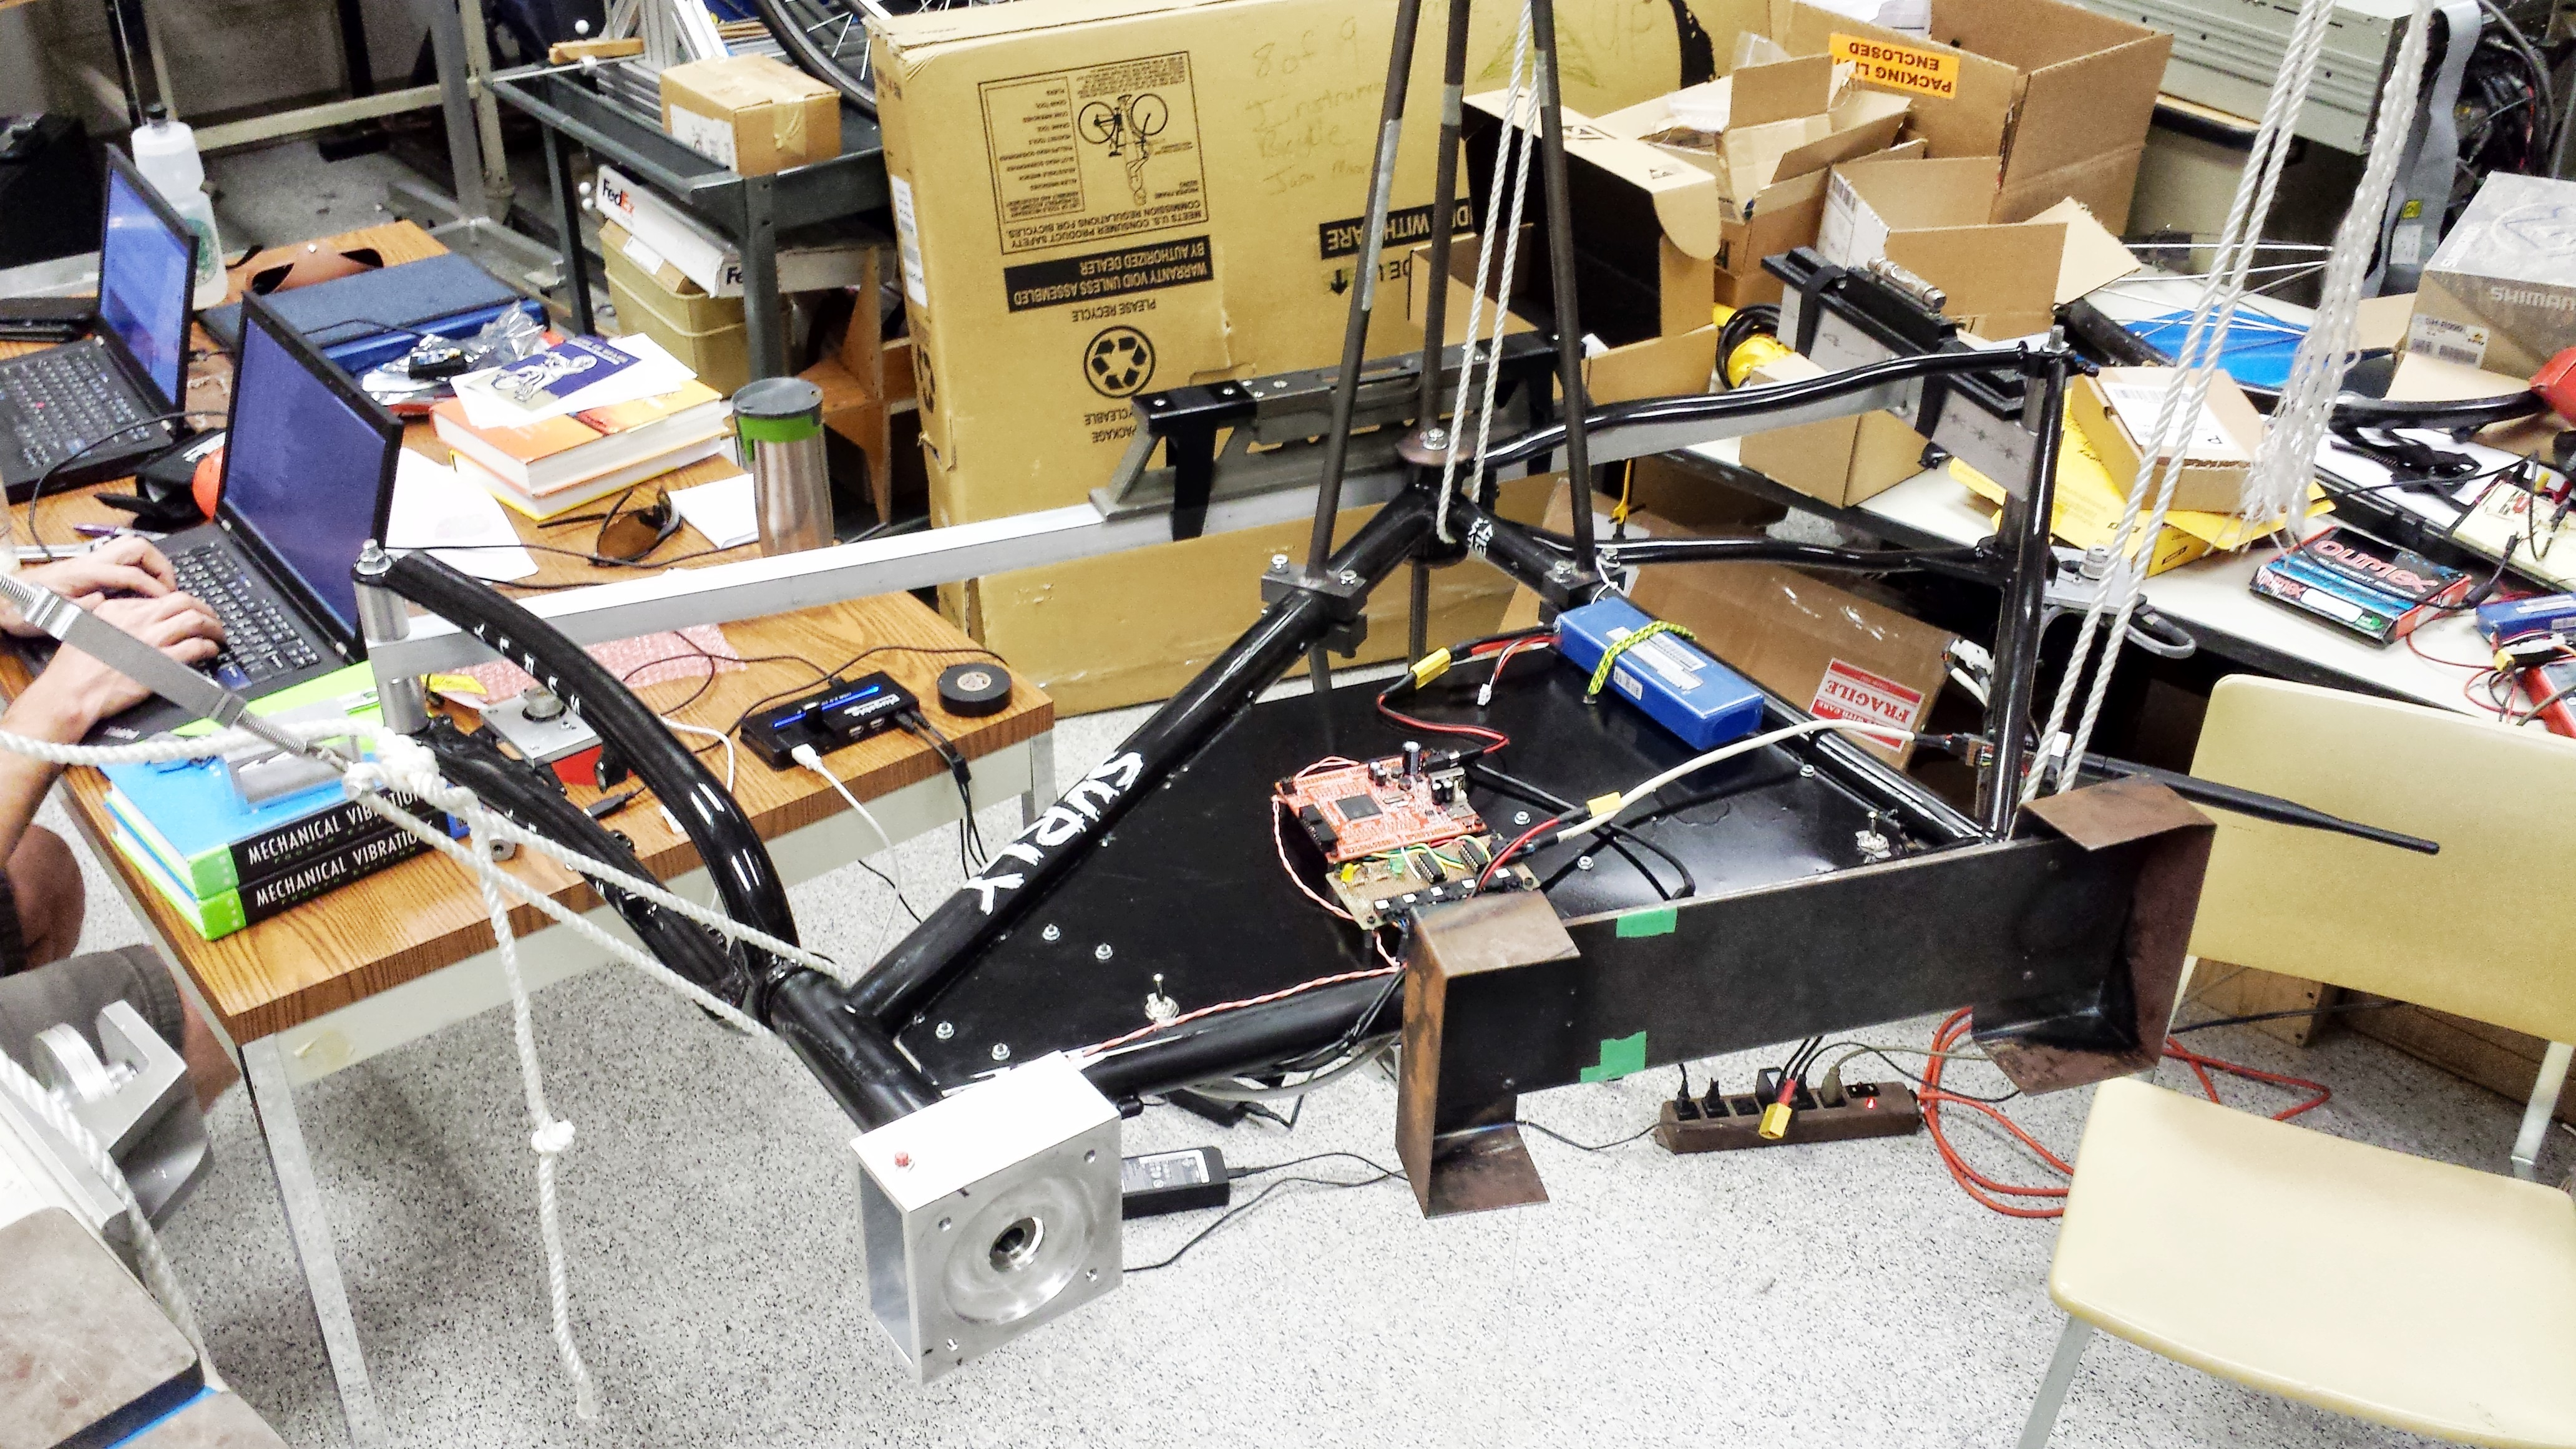
\includegraphics[width=\textwidth]{images/20130711_163732_2.jpg}
  \caption{Calibration of steer angle encoder, accelerometer, and rate
    gyroscope ($\phi=-\pi/2$ configuration). The steer calibration fixture
    ensured $\delta=0$ and provided surfaces to rest the bubble levels (visible
    on far side of bicycle frame). Two turnbuckles were used to make minor
  orientation adjustments to level the frame (visible on left side of image).}
  \label{rb:img:calibration}
\end{figure}

A combined rate gyroscope and accelerometer MEMS
sensor~\cite{InvensenseMPU6050} was fixed to the underside of the battery pack
plate as shown in \autoref{rb:img:imuplacement}. The gyroscope and
accelerometer sensor axes were assumed to be aligned with each other since they
are manufactured on the same piece of silicon. The sensor $\bm{s}_x-\bm{s}_y$
plane was approximately parallel to the plane of the battery plate, with
$\bm{s}_y$ pointed approximately forward, $\bm{s}_y$ to the left, and
$\bm{s}_z$ down.

As described in Chapter 1, the bicycle model introduces set of dextral unit
vectors fixed to the rear frame $R$ of the bicycle, with $\bm{r}_z$ parallel to
the steer axis and down, $\bm{r}_y$ perpendicular to the frame plane and to the
right, and $\bm{r}_x = \bm{r}_y \times \bm{r}_z$ ($\bm{r}_x$ points forward and
slightly up when the bicycle is in the reference configuration). Fixed to the sensor $S$
are a set of dextral unit vectors with $\bm{s}_x$ and $\bm{s}_y$ in the plane
of the integrated circuit, and $\bm{s}_z$ normal to the plane of the integrated
circuit. To orient the sensor relative to the bicycle, first align $S$ with
$R$, then apply the following successive body-fixed ZXY rotations: $\alpha -
\pi/2$, $\beta$, $\gamma$. The first rotation was offset by $-\pi/2$ so that
all three angles were near zero.

\begin{figure}[ht]
  \centering
  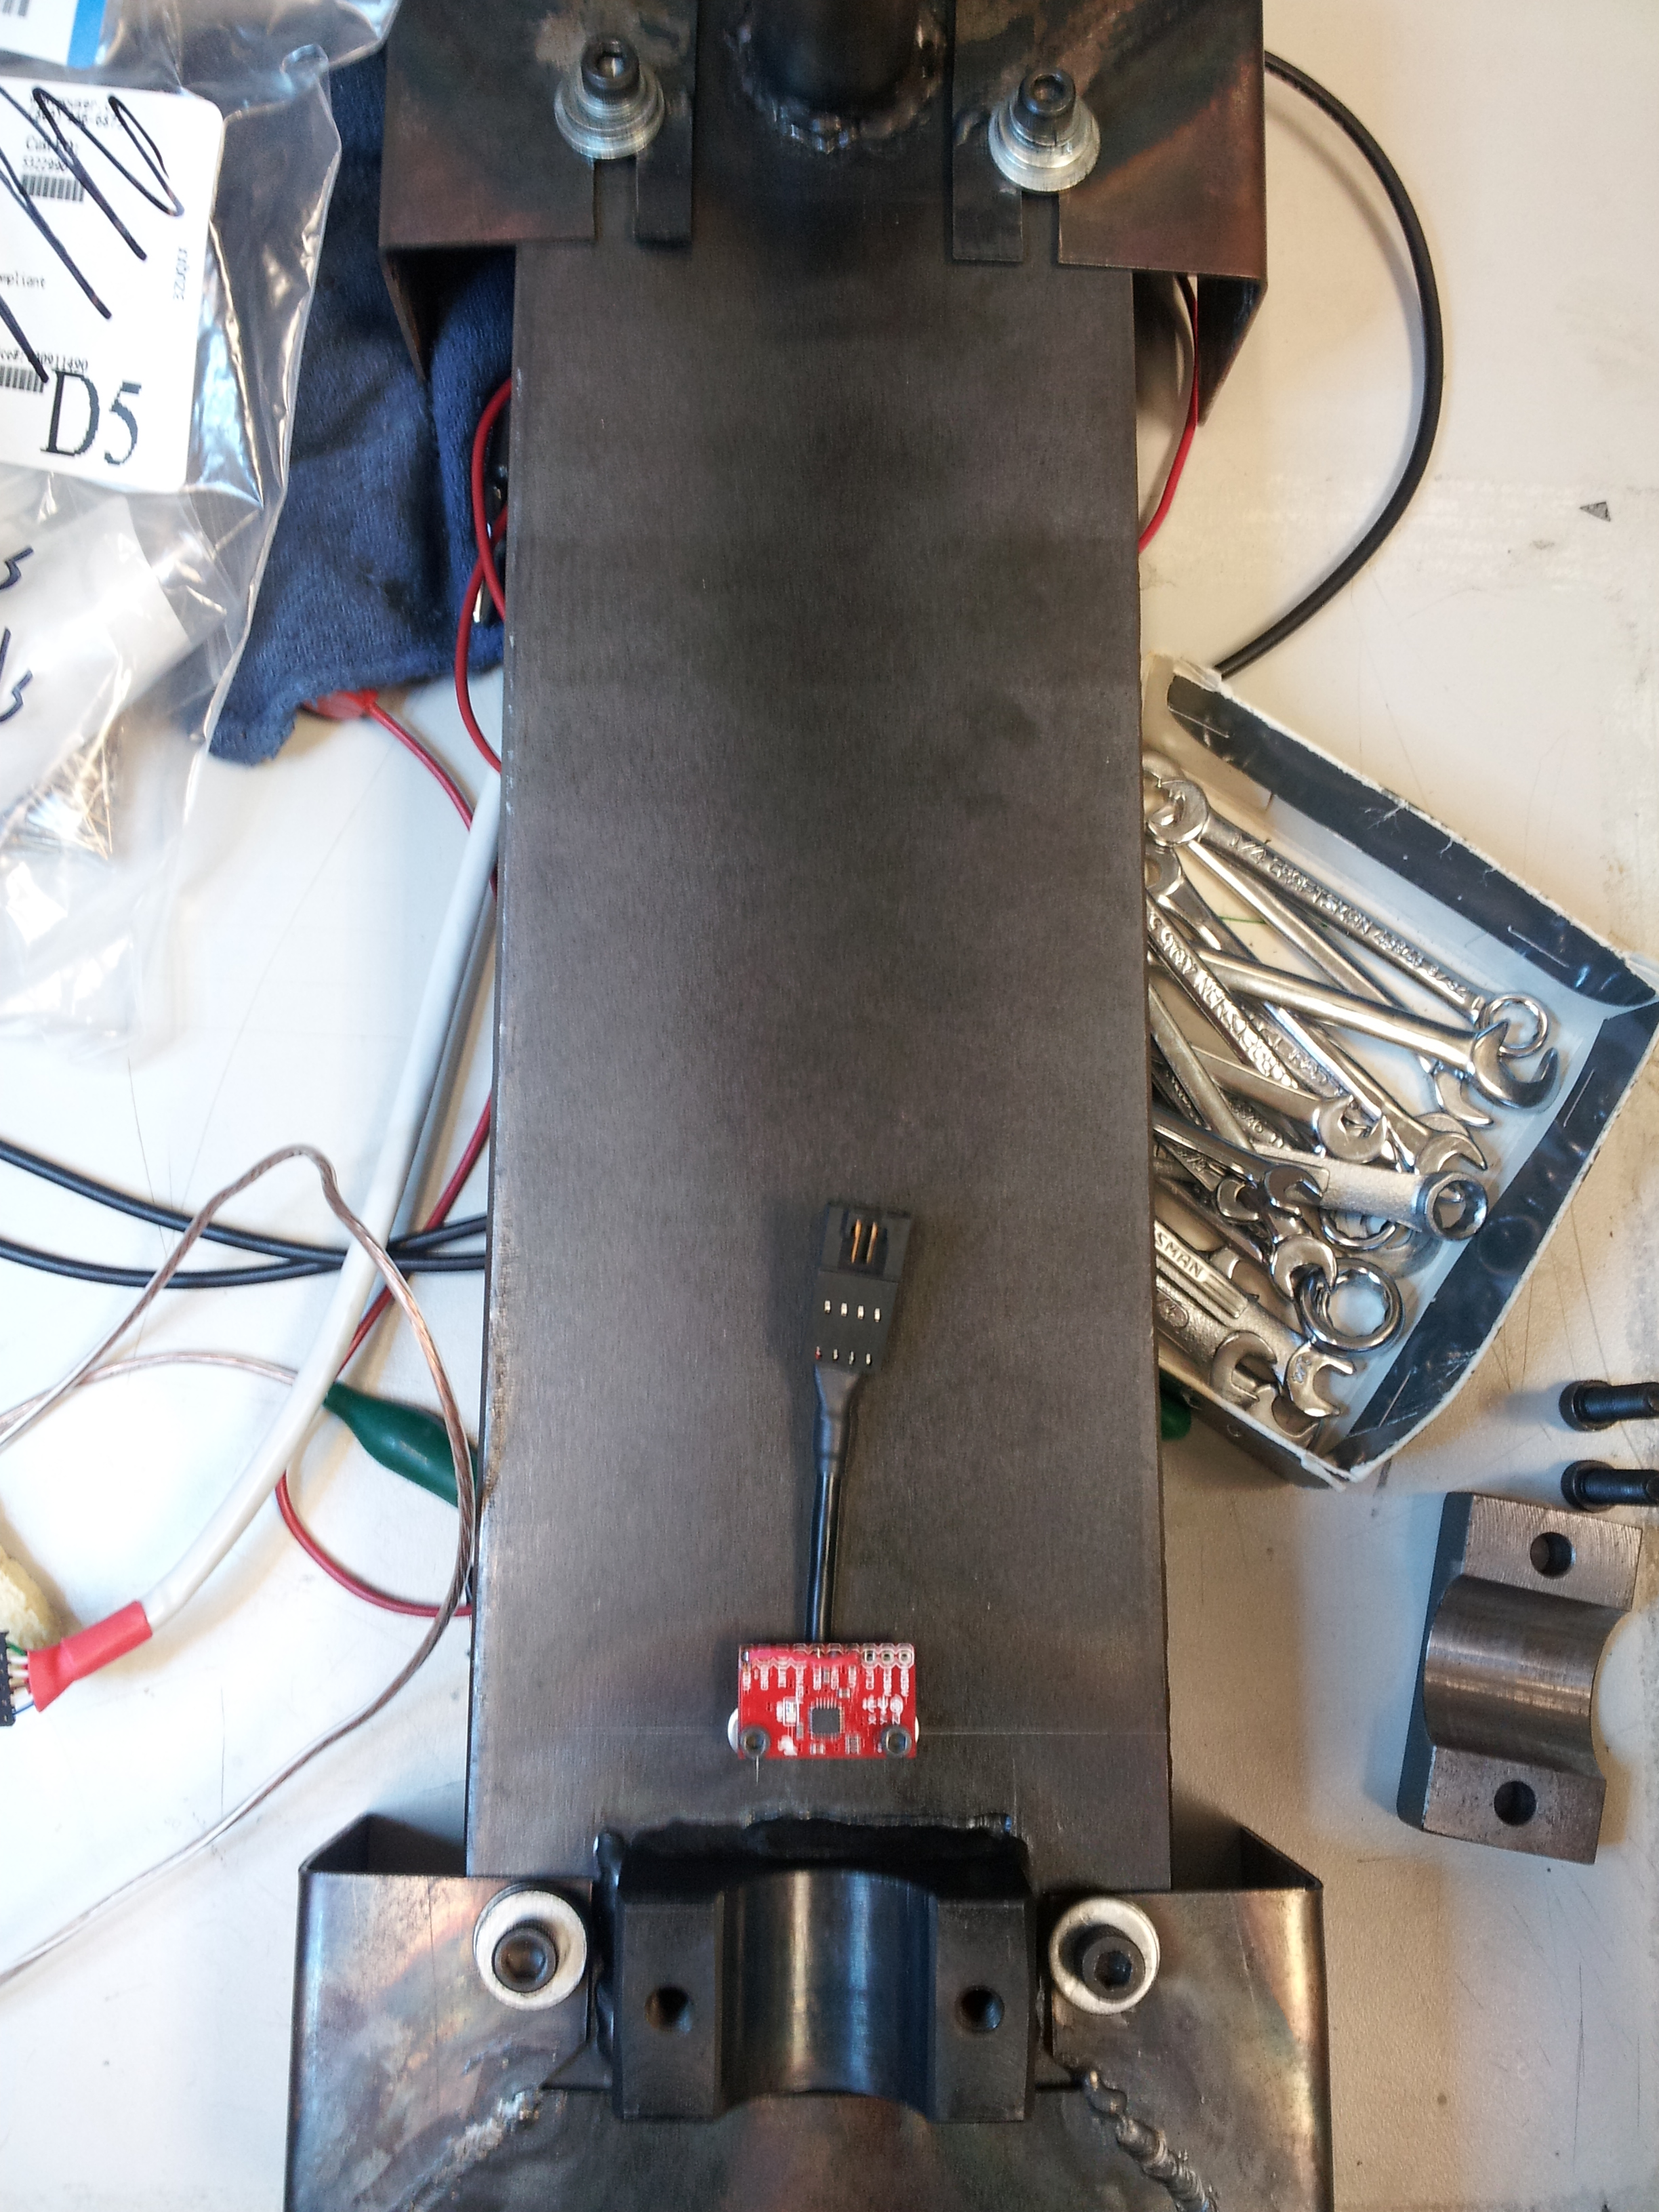
\includegraphics[width=.6\textwidth,angle=90]{images/IMG_20130325_195226.jpg}
  \caption{Rate gyroscope and accelerometer sensor placement on bottom of
  battery support plate. The top tube clamshell bracket is visible on the right side of
the image (forward end of battery plate). On the left side of the image the
seat post is partially visible. The mounting hardware for the battery box is also
visible.}
  \label{rb:img:imuplacement}
\end{figure}

To determine the three angles $\alpha$, $\beta$, and $\gamma$, the static
acceleration was measured in three sensor directions ($\bm{s}_x$, $\bm{s}_y$,
$\bm{s}_z$) in six unique orientations. The six orientations are those that
would be obtained if $R$ were aligned with and fixed to the edges of a perfect
cube and the cube was laid on a level surface on each of its six sides.  These
six configurations correspond to the following bicycle orientations:
$\phi=\pm\pi/2$ (frame plane horizontal), $\phi=0$ and $\theta_R = \{-\pi/2, 0,
\pi/2, \pi\}$ (frame plane vertical, two horizontal steer axis orientations and
two vertical steer axis orientations). The sensed acceleration in the three sensor
directions was recorded for approximately sixty seconds while the bicycle was
in each orientation.

The six orientations were obtained by suspending the bicycle by ropes from
three points of attachment and using a turnbuckle on two of the ropes to level
the desired surface in two directions. Two precision horizontal bubble levels
were attached to the frame 90 degrees apart to permit levelling in both
directions.  Once levelled, the bicycle was left to rest for approximately 5
minutes to allow for small swinging and twisting oscillations to die out; this
was also aided by suspending a weight from the frame with fishing line and
hanging it into a bucket of water. The bucket of water provided some
dissipation which helped damp out vibrations. Once stationary (within the
limits of the vibrating building), data collection was initiated.

When at rest, the accelerometer senses the gravitational field as if it were
accelerating \textit{upwards} at $g$, this corresponds to $-g\bm{n}_z$.
Resolving $-g\bm{n}_z$ into the three sensor measurement directions yields
\begin{align}
  \label{rb:eq:imux}
-g\bm{n}_z \cdot \bm{s}_x &= g \left(- s_{\alpha}
s_{\beta} s_{\gamma}
s_{\phi} + s_{\alpha}
s_{\theta} c_{\gamma}
c_{\phi} + s_{\beta}
s_{\gamma} s_{\theta}
c_{\alpha} c_{\phi} +
s_{\gamma} c_{\beta}
c_{\phi} c_{\theta} +
s_{\phi} c_{\alpha}
c_{\gamma}\right) \\
%
  \label{rb:eq:imuy}
-g\bm{n}_z \cdot \bm{s}_y &= g \left(- s_{\alpha}
s_{\phi} c_{\beta} -
s_{\beta} c_{\phi}
c_{\theta} + s_{\theta}
c_{\alpha} c_{\beta}
c_{\phi}\right) \\
%
  \label{rb:eq:imuz}
-g\bm{n}_z \cdot \bm{s}_z &= g \left(s_{\alpha}
s_{\beta} s_{\phi}
c_{\gamma} + s_{\alpha}
s_{\gamma} s_{\theta}
c_{\phi} - s_{\beta}
s_{\theta} c_{\alpha}
c_{\gamma} c_{\phi} +
s_{\gamma} s_{\phi}
c_{\alpha} - c_{\beta}
c_{\gamma} c_{\phi}
c_{\theta}\right)
\end{align}
Where $s_{x}$ and $c_{x}$, $x=\alpha,\beta,\gamma,\phi,\theta$ are
abbreviations of $\sin{x}$ and $\cos{x}$. The goal of the calibration was to
convert the measured acceleration to the true acceleration, and for this reason
the following slightly non traditional (yet equally representative) form of the
acceleration sensor model was used
\begin{align}
  \label{rb:eq:sensormodel}
  \left[
    \begin{matrix}
      -g\bm{n}_z \cdot \bm{s}_x \\
      -g\bm{n}_z \cdot \bm{s}_y \\
      -g\bm{n}_z \cdot \bm{s}_z
    \end{matrix}
  \right]
  &=
  \left[
    \begin{matrix}
      S_{xx} & S_{xy} & S_{xz}\\
      S_{xy} & S_{yy} & S_{yz}\\
      S_{xz} & S_{yz} & S_{zz}
    \end{matrix}
  \right]
  \left[
    \begin{matrix}
      a_{x} \\
      a_{y} \\
      a_{z}
    \end{matrix}
  \right]
  +
  \left[
    \begin{matrix}
      b_{x} \\
      b_{y} \\
      b_{z}
    \end{matrix}
  \right]
\end{align}
where $a_x, a_y, a_z$ are the raw sensor measurements (in units of bits), $b_x,
b_y, b_z$ are biases (in units of m/s$^2$), $S_{xx}, S_{yy}, S_{zz}$ are the
sensitivities, and $S_{xy}, S_{yz}, S_{xz}$ are the cross axis sensitivities,
both of which have units of m/s$^2$/bit. Cross axis sensor symmetry was
assumed, i.e., $S_{xy} = S_{yx}$.

Equating the right side of Equations \ref{rb:eq:imux}-\ref{rb:eq:imuz} with the
right side of \autoref{rb:eq:sensormodel}, evaluating at the value of lean
$\phi$ and pitch $\theta$ corresponding with a particular configuration, and
taking the time series mean of each of the raw measurements $a_x, a_y, a_z$, we
obtain three equations with twelve unknowns. Repeating for each of the six
configurations, we obtain an overdetermined system of eighteen equations in
twelve unknowns. The twelve unknowns are the six sensitivities, the three
biases, and the three orientation angles relating the sensor frame to the
bicycle frame. This overdetermined system of equations was solved by the method
of least squares to obtain the following sensitivities, biases, and orientation
angles
\begin{align}
  \left[
    \begin{matrix}
      S_{xx} \\
      S_{yy} \\
      S_{zz} \\
      S_{xy} \\
      S_{yz} \\
      S_{xz}
    \end{matrix}
  \right]
  &=
  \left[
    \begin{matrix}
      \num{5.9898e-4} \\
      \num{5.9534e-4} \\
      \num{5.8288e-4} \\
      \num{-5.4766e-7} \\
      \num{-1.6455e-6} \\
      \num{1.9272e-6}
    \end{matrix}
  \right] \text{m/s$^2$/bit} \\
  \left[
    \begin{matrix}
      b_{x} \\
      b_{y} \\
      b_{z}
    \end{matrix}
  \right]
  &=
  \left[
    \begin{matrix}
      -0.5700 \\
       0.0514 \\
       1.1690
    \end{matrix}
  \right] \text{\si{m/s^2}} \\
  \left[
    \begin{matrix}
      \alpha \\
      \beta \\
      \gamma
    \end{matrix}
  \right]
  &=
  \left[
    \begin{matrix}
      0.0031 \\
      0.3230 \\
     -0.0182
    \end{matrix}
  \right] \text{rad}
\end{align}
The diagonal entries of $S$ were very close to the manufacturer specified
sensitivity of \num{5.9876e-4} m/s$^2$/bit. The diagonal entries were greater than
the off-diagonal entries by more than two orders of magnitude, indicating the
cross axis sensitivity was less than 1\%, also in line with the manufacturers
specifications. The means of three rate gyroscope measurements axes were
computed for each static configuration, and were found to be independent of
configuration (as expected). These means were used as biases for the
measurement of the bicycle frame angular velocity and were found to be
\begin{align}
  E[\omega_x] &= -0.1204\text{ rad/s}\\
  E[\omega_y] &=  0.0316 \text{ rad/s}\\
  E[\omega_z] &=  0.0100 \text{ rad/s}
\end{align}
Since a rate table or other convenient means of calibrating the gyroscope
sensitivities was not available, the manufacturer published gyroscope
sensitivities were used.

\subsection{Actuators} \label{rb:subsec:actuators}
The robot bicycle was equipped with a rear wheel hub motor to drive the rear
wheel and a fork motor to steer the bicycle. Both motors were brushless DC
motors and were interfaced to the microcontroller with Copley Controls digital
motor drives (fork: ACJ-055-18~\cite{CopleyACJ}, rear wheel:
ADP-090-36~\cite{CopleyADP}). Both digital motor drives were configured in
current control mode and internally implemented a PI current (with gains
automatically selected via manufacturer software based upon motor parameters)
controller that operated at 30kHz. The current commands were generated by the
microcontroller as 3.3V pulse width modulated (PWM) signals which were
converted by the motor drives to the appropriate high voltage, high current PWM
signals to the motor windings. The bicycle control system was designed to
generate applied joint torques as control signals, which were then scaled by
the respective motor torque constants before generating the current command PWM
signal.

The rear wheel was built with an electric hub motor~\cite{AmpedBikes}. The
manufacturer supplied rim and spokes were of extremely low quality (very weak,
untrue, and noticeably inertially non-symmetric), so they were replaced with DT
Swiss 2.0mm stainless steel spokes and Mavic model A719, 700c diameter, 36 hole
rim. The rear hub axle served as the motor stator and armature with the three
motor power leads exiting the left side of the axle. The motor field magnets
were fixed to the inside of the hub shell and rotated along with the spokes,
rim, and tire when current was applied to the motor windings. This motor
configuration is commonly known as the ``outrunner'' configuration. No
manufacturer specifications were available for this motor, so the motor torque
constant was determined experimentally by applying a constant rear wheel
current $I_R$ with while the wheel was off the ground and measuring the angular
response. The spin inertia $J_r$ of the rear wheel was measured
(\autoref{rb:subsec:parameters}), and the idealized DC motor equation
$J_r\ddot{\theta}_R = K_t I_r$ was integrated twice with respect to time
(constant current assumed and $\theta_R(0)=\dot{\theta}_R(0) = 0$) to obtain
$\theta = \frac{K_t I_r}{2J_r}t^2$. A least squares fit was then used to
estimate $K_t=6.6$ Nm/A. Since a PI speed controller was implemented to control
rear wheel rate, it was not critical to know $K_t$ precisely (PI controllers
perform reasonably well even when system parameters are not well known); for
this reason we didn't expend any effort to more accurately determine $K_t$.

The fork motor~\cite{TeknicM3441} was bolted to an aluminum box section which
in turn was bolted to a custom upper headset. The custom upper headset was
pressed into the upper end of the bicycle steer tube with green Loctite to
ensure it would not twist relative to the frame when motor torques were
applied. In contrast to the rear wheel hub motor, the fork motor stator and
armature windings were fixed to the outer portion of the motor (fixed to the
bicycle frame) and the field magnets were fixed to the motor output shaft.  The
motor output shaft was equipped with a key-way which was mated to a circular
plug fixed to the inside of the steer tube. The circular plug was rigidly
attached to the steer tube in the same way a threaded bicycle stem wedge
expander attaches to the bicycle steer tube. The upper portion of the circular
plug (which mates with the motor shaft) was bored with a hole to match the
diameter of the motor output shaft, and an internal key-way was cut with a
wire-cut electrical discharge machine. Once the motor was secured, a set
screw was threaded into the upper portion of the plug to make contact with the
motor key. This design permitted the fork to be driven directly by the motor
without the use of a gearbox, and still permitted the motor to be removed
easily if necessary. Most importantly, the design had no backlash between the
motor shaft and the fork. A previous design was attempted which made use of a
precision gearbox, but it was found to have unacceptable levels of backlash.
Since the sign of the steer angle rate frequently changes during normal
operation of a bicycle, any backlash between the motor fork is extremely
undesirable.

\subsection{Batteries} \label{rb:subsec:batteries}
Four 12.0V sealed lead acid (SLA) batteries were wired in series and used to
power the motors and the digital motor drives. The SLA batteries were arranged
in a row of four and tightly bound to each other with duct tape and nylon
strapping. All other electronics were powered with a two-cell 7.2V lithium
polymer battery~\cite{Zippy5000} which was fastened to the right side of the
electrical panel with velcro and a small bungee cord.

The SLA batteries were securely fastened to the bicycle frame with a
1/4''x4''x18'' steel plate to support the bottom of the batteries, and a sheet
metal box on either end of the plate to maintain the lateral and longitudinal
position of the batteries on the relative to the plate. The plate was rigidly
attached to the bicycle frame with a steel seat post on the rear end and a
steel top tube bracket on the forward end. The seat post and bracket were
welded to the bottom of the plate such that when the seat post was inserted
into the frame, the top tube bracket interfaced with the top of the top tube to
align the steel plate symmetrically with respect to the bicycle frame. The top
tube bracket was a clamshell design, with the top half welded to the bottom of
the steel plate and the bottom half placed on the underside of the top tube and
then bolted to the top half, thereby securing the plate to the tube (see
\autoref{rb:img:imuplacement}). When the bicycle was in the upright reference 
configuration, the battery plate was approximately horizontal. In addition to
the battery box to maintain the lateral and longitudinal position of the
batteries with respect to the frame, nylon straps were used to secure the
batteries onto the plate.

\subsection{Wireless communication} \label{rb:subsec:wireless}
A pair of XBee Pro~\cite{XBeePro} wireless radios were used as a serial cable
replacement between the robot bicycle and a nearby laptop computer. Commands
were sent to the robot bicycle by typing them into a serial terminal
program~\cite{moserial} which transmitted the text as a simple character stream
through the USB port of the computer to the XBee Pro radio, which in turn
transmitted the commands wirelessly. A shell thread running on the robot
bicycle microcontroller monitored the serial port for received commands along
with optional command arguments. When a valid command was received, the
corresponding function was executed. A list of available commands are detailed
in \autoref{rb:subsec:ui}.


\section{Control system design} \label{rb:sec:control}
This section details the theoretical framework as well as the implementation
details of the control system for the robot bicycle. Lower level details and
user interface considerations are detailed in \autoref{rb:subsec:data} and
\autoref{rb:subsec:ui}.

\subsection{Data logging} \label{rb:subsec:data}
Data was written at 200Hz, in binary format, to a single file per ``run'' on
the micro SD card. The data format used Google Protocol
Buffers~\cite{GoogleProtoBuf}, a platform independent data interchange format
used by Google. In addition to abstracting away platform dependent issues (byte
order, word size, etc.), this data format permitted data fields to be marked as
required or optional, and new data fields could be easily added without losing
the ability to easily work with old data collected without the new fields; this
ensured backwards compatibility for all data collected during the development
and refinement of the control system. This feature proved essential for
debugging errors and being able to inspect intermediate calculations during an
experiment to verify that we had implemented the control algorithms correctly.

The following is a partial list of the data that was recorded during each run;
the complete list is viewable in the source code.
\begin{description}
  \item[System time] Units of 0.25$\mu$s. Time elapsed since the beginning of
    data collection.
  \item[Computation time] Units of 0.25$\mu$s. Time elapsed from the
    beginning of each 5ms period until data collection and logging are
    complete. Used to ensure no calculations exceed the loop time.
  \item[System state] 32-bit unsigned integer whose bits are set high or low
    depending on the Boolean state of the following: Rear motor enable, steer
    motor enable, rear motor fault, steer motor fault, sample buffer
    encode/initialization/overflow error, hardware button
    (\autoref{rb:subsec:sensors}), IMU communication error, filesystem error.
  \item[Rear wheel and steer angles and rates] Units of rad, rad/s. Rear wheel
    angle and angular rate, steer angle and angular rate. Rear wheel angular
    rate was determined by a 100ms moving average of an ideal derivative
    ($\dot{\theta}_R \approx \Delta\theta_R / \Delta t$), steer angular rate
    was obtained by a low pass filtered ideal derivative ($G(s)=s/(s+20\pi)$).
    This difference was necessary because the discretization error of the rear
    wheel encoder was 2 orders of magnitude higher than that of the steer
    encoder.
  \item[Commanded rear wheel rate and yaw rate] Units of rad/s. By
    default, these both start at 0 rad/s and change once the \verb|speed| or
    \verb|yaw_rate| commands are issued. Speed was specified in m/s but
    converted to rear wheel rate by dividing by rear wheel radius.
  \item[Motor torques] Units of Nm. The torque commanded by rear motor
    controller and the fork motor controller. Each signal was divided by the
    respective motor torque constant to calculate the current command in units
    of Amperes.
  \item[Frame angular velocity, sensor acceleration] Units of rad/s, m/s$^2$.
    Both quantities were computed by applying the sensitivities, biases, and
    direction cosine matrix to map raw measurements to appropriately scaled
    measurments in the bicycle body-fixed frame.
    (\autoref{rb:subsec:sensors}).
\end{description}


\section{Feedback control system}
Two independent control systems were implemented: A rear wheel rate controller
and a yaw rate controller. The \verb|speed| command was used to change the
commanded rear wheel rate, while the \verb|yaw_rate| command was used to change
the commanded yaw rate.

\subsection{Rear wheel rate controller} \label{rb:subsec:rw_control}
The rear wheel rate controller was a discrete time proportional-integral (PI)
controller with conditional integration. Whenever the desired rear
wheel torque command exceeded the allowable torque, it was saturated and the
integrator state was not updated. This technique prevented integrator windup
and was simple to implement. The control law was
\begin{align}
  e_i &= \dot{\theta}_{R,i,\text{commanded}} - \dot{\theta}_{R,i} \\
  \tau_{i,\text{desired}} &= K_p e_i + x_{i-1}\\
  x_{i} &= \left\{
      \begin{matrix}
        x_{i-1} + \frac{K_p e_i (t_i - t_{i-1})}{T_i} & \text{if } |\tau_{i,\text{desired}}| \leq \tau_{\text{max}} \\
        x_{i-1} & \text{if } |\tau_{i,\text{desired}}| > \tau_{\text{max}}
      \end{matrix}
    \right. \\
  \tau_{i} &= \text{sat}(\tau_{i, \text{desired}}, \tau_{\text{max}})
\end{align}
where $x_{i}, \tau_{i,\text{desired}}$, and  $\tau_{i}$ are the integrator
state, the desired rear wheel torque, and the saturated rear wheel torque,
respectively, all for time step $i$. The maximum torque was limited by the
maximum current of the digital motor drive, $\tau_{\text{max}}$ = 158Nm (the
max motor current was configured to be 24.0A, and a rear motor torque was
estimated to be 6.6Nm/A). Through repeated experimentation, we found that a
gain of $K_p =50$ and an integration time constant of $T_i = 2000$ provided
sufficiently fast response, no steady state tracking error, and no noticeable
oscillatory behavior that can be present when integral action is used.

\subsection{Yaw rate controller} \label{rb:subsec:yr_control}
The yaw rate controller was implemented with an inner loop and an outer loop.
The inner loop was comprised of a full state estimator for the four bicycle
states using measurements of steer angle $\delta$ and lean rate $\dot{\phi}$,
and a full state feedback control law which used the state estimates instead of
the states. The stabilized inner loop was then inserted into an outer yaw rate
control loop which computed an additive control action based upon the error
between the commanded yaw rate $\dot{\psi}_c$ and the estimated yaw rate
$\dot{\hat{\psi}}$.  The block diagram for the complete system is shown in
\autoref{rb:fig:yr_block_diagram}. An additive sinusoidal disturbance torque
with user selectable amplitude $a_d$ and frequency $f$ (see the \verb|disturb|
command in \autoref{rb:subsec:ui}) was also incorporated into the design; by
default $a_d=0$ so that no disturbance was applied unless requested by the
user.

\begin{figure}[h]
  \centering
  \begin{tikzpicture}[
    block/.style={rectangle,draw,thick,minimum height=2em,minimum width=2em},
    sum/.style={circle,draw,thick,inner sep=0pt,minimum size=4mm},
    connector/.style={->,thick},
    guide/.style={},
    line/.style={thick}]
    % We start by placing nodes in a 5x10 matrix
    \matrix[ampersand replacement=\&, row sep=0.2cm, column sep=0.4cm] {
    %\node (disturbance_input) [coordinate, above=of inner_sum] {};
    % First row
    \node (input) [] {$\dot{\psi}_c$}; \&
    \node (outer_sum) [sum,label=135:$+$,label=225:$-$] {}; \&
    \node (pi_block) [block] {PI}; \&
    \node (inner_sum) [sum,label=45:$+$,label=135:$+$,label=225:$+$] {}; \&
    \&
    \node (branch_1) [coordinate] {}; \&
    \node (bicycle_block) [block,label=above:Bicycle dynamic model] {
    $\begin{aligned}\dot{x} &= Ax + B\tau_\delta\\
                          y &= C x
                        \end{aligned}$}; \& \& \& \\
    % Second row
    \& \& \& \& \& \node (u_route1) [coordinate] {}; \& \& \node (u_route2)
    [coordinate] {}; \& \node(y_route) [coordinate] {}; \& \\
    % Third row
    \& \& \& \& \node (gain_block) [block] {$K$}; \& \node(branch_2)
    [coordinate] {}; \&
    \node (estimator_block) [block,label=below:State estimator] {%
      $\dot{\hat{x}} = (A - LC)\hat{x} + B\tau_\delta + Ly$}; \& \& \& \\
    % Fourth row
      \& \& \node(C_yr) [block] {$C_{\dot{\psi}}$}; \& \& \& \& \& \& \& \\
    };
    % Place disturbance node above inner_sum, not using the matrix layout
    \node (disturbance) [above=of inner_sum] {$d = a_d\sin(2\pi f t)$};

    \draw[connector] (input.east) to (outer_sum.west);
    \draw[connector] (outer_sum.east) to node[auto] {$e_{\dot{\psi}}$} (pi_block.west);
    \draw[connector] (pi_block.east) to node[auto] {$r$} (inner_sum.west);
    \draw[connector] (disturbance.south) to (inner_sum.north);
    \draw[connector] (inner_sum.east) to node[auto] {$\tau_\delta$} (bicycle_block.west);
    \draw[connector] (estimator_block.west) to node[auto,swap] {$\hat{x}$} (gain_block.east);
    \draw[connector] (gain_block.west) -| node[auto] {$u$} (inner_sum.south);
    \draw[line] (branch_1) to (u_route1) to (u_route2);
    \draw[connector] (u_route2) |- ($(estimator_block.east) + (0mm, 1.5mm)$);

    \draw[line] (bicycle_block.east) -| node[auto] {$y$} (y_route);
    \draw[connector] (y_route) |- ($(estimator_block.east) - (0mm, 1.5mm)$);

    \draw[connector] (branch_2) |- (C_yr.east);
    \draw[connector] (C_yr.west) -| node[auto] {$\dot{\hat{\psi}}$} (outer_sum.south);

  \end{tikzpicture}
  \caption{Yaw rate control block diagram. The bicycle state is $x=[\phi,
  \delta, \dot{\phi}, \dot{\delta}]$, $\hat{x}$ is the state estimate, input to
  the bicycle is steer torque $\tau_\delta$, the measurements are $y =
  [\delta, \dot{\phi}]$.}
  \label{rb:fig:yr_block_diagram}
\end{figure}
The state feedback gain $K$ was computed by discretizing the plant model and
solving the discrete algebraic Riccati equation associated with the cost
function
\begin{align}
  J &= \sum_{i=1}^{\infty} (x_i^T Q x_i + u_i^T R u_i)
\end{align}
where $Q$ and $R$ were selected to be
\begin{align}
  Q &= \text{diag}(\frac{1}{(\frac{2\pi}{180})^{2}},
                   \frac{1}{(\frac{5\pi}{180})^{2}},
                   \frac{1}{(\frac{2\pi^2}{180})^{2}},
                   \frac{1}{(\frac{100\pi^2}{180})^{2}}) \\
  R &= \frac{1}{0.5^2}
\end{align}
This choice was selected following Bryson's rule~\cite{Bryson1975}; the terms
inside the $(\cdot)^2$'s in the denominator can be viewed as the ``maximum
allowable'' value for the corresponding state or control variable (e.g., the
``maximum allowable'' value for lean $\phi$ was $\frac{2\pi}{180}=2^{\circ}$).

Once the state feedback gain was computed, the closed loop eigenvalues of the
stabilized plant dynamics $A+BK$ were computed, and the estimator gain was
selected using pole placement. The poles of the estimator were all placed on
the negative real axis, equally spaced by 0.2 rad/s, and with the slowest estimator
pole being $3\min(\text{Re}(\sigma(A+BK)))$. This ensured the convergence of
the estimator was substantially faster than the controller dynamics.

With the bicycle dynamics stabilized by the inner loop, an outer loop was added
to track yaw rate. Yaw rate was chosen as the variable to track because it is a
natural way to describe both straight line motion ($\dot{\psi}=0$) as well as
steady turning motion ($\dot{\psi}=c\ne0$). The Matlab function
\verb|pidtune()| was used to compute the PI gains.

Since the dynamics of the bicycle vary with speed, this control system design
was performed at 101 speeds, logarithmically spaced between 0.5m/s and 10m/s.
All matrices in \autoref{rb:fig:yr_block_diagram} were output to a C++ file as
a sorted array of matrices parameterized by speed. This file was then compiled
into the firmware and gain scheduling was used to compute the actual control
law based on the measured speed. During a experimental run, the measured speed
was used to perform a binary search into the array to find the matrices
associated with speeds bounding the measured speed. A linear interpolation of
the state update and control law were performed using these nearest two speeds.
An implication of this is that estimation and control was not possible below
0.5m/s. This turned out not to be a problem as long as the bicycle was started
from a standstill near the upright reference configuration.

\subsection{User interface} \label{rb:subsec:ui}
The following list details the available commands and gives a brief description
of each.

\begin{description}
  \item[\Q{collect [filename]}] Begin main data collection and control loop and store
    data in optional argument \verb|filename| (if not supplied, data is stored in
    \verb|samples.dat|).
  \item[\Q{disable}] Immediately disable the motors and end data collection.
  \item[\Q{reset}] Perform a software reset of the microcontroller.
  \item[\Q{threads}] Show the memory address, stack address, priority, number
    of references to this thread, thread state, thread time in ticks, and the
    name of all currently running threads.
  \item[\Q{calibrate}] Begin the steer angle calibration routine (see
    \autoref{rb:subsec:sensors})
  \item[\Q{homefork}] Wait for the steer encoder index signal to set the steer calibration offset.
  \item[\Q{e_thresh v_e}] Set state estimation threshold speed to \verb|v_e| m/s.
    \verb|v_e| must be greater than or equal to 0.5m/s (the lowest speed
    for which linearized bicycle dynamics state space matrices were generated).
  \item[\Q{c_thresh v_c}] Set the threshold speed to \verb|v_c| m/s. Once the
    bicycle speed \verb|v| exceeds \verb|v_c| yaw rate control is enabled. Must
    be larger than estimation threshold speed.
  \item[\Q{thresh v_e v_c}] Simultaneously set state estimation and control threshold speeds.
  \item[\Q{disturb a_d f}] Set disturbance amplitude to \verb|a_d|\num{1e-2}Nm
    and disturbance frequency to \verb|f| Hz (see
    \autoref{rb:fig:yr_block_diagram}).
  \item[\Q{speed v}] Set commanded speed in m/s. The control system will
    immediately attempt to track this speed until a fault occurs or the
    reference is changed by the user. On reset, the reference speed is set 0
    m/s.
  \item[\Q{speed_limit v d}] Set commanded speed to \verb|v| m/s and distance
    limit to \verb|d| meters. This works the same as \verb|speed| except that
    once the bicycle has travelled \verb|d| meters, the commanded speed is
    changed to 1.0 m/s, a speed which was easy to walk next to and catch the
    bicycle.
  \item[\Q{l_thresh t}] Set the lateral acceleration threshold to \verb|t|. At
    the beginning of each run, a green LED is illuminated when the bicycle
    lateral acceleration is below \verb|t| (with a default of \verb|t|=0.01
    m/s$^2$). This enables the bicycle to be initialized with as close to zero
    lean angle as possible. The sensed lateral acceleration is non-zero in
    static conditions because the accelerometer senses the gravitational field.
  \item[\Q{yaw_rate yr}] Set the commanded yaw rate in rad/s. On
    reset, reference yaw rate is 0 rad/s (straight line motion).

\end{description}

\section{Results} \label{rb:sec:experiments}

\subsection{Experiments conducted} \label{rb:subsec:experiments}
On July 13, 2013, twenty eight experimental runs were performed on the Dairy
Road basketball courts of the UC Davis campus (38.53794$^{\circ}$ North,
121.759475$^{\circ}$ West). Oliver Lee and Dr. Mont Hubbard were stationed at the
northeast corner of the east court, while I travelled east and west with the
robot bicycle each run. To begin each run, Oliver Lee operated the laptop and
issued commands to configure the filename (following a naming convention $<$run
number$>$.dat), speed set point, distance to travel before reducing the speed
set point to 1.0 m/s, and optionally, an additive sinusoidal disturbance steer
torque of magnitude $a_d$ cNm and frequency $f_d$ Hz. Dr. Hubbard took notes
about each run and coordinated with Oliver Lee to ensure commands issued to robot
were consistent with his notes. Prior to issuing a non-zero speed set point
command, I held the bicycle near the reference configuration (as indicated by
two LED's which turned on when IMU lateral acceleration and steer angle were
less than 0.01 m/s$^2$ and 1.0 deg, respectively), then ran along side the
bicycle as it travelled east to west or west to East. At the end of each run, I
would turn of the main power switches to each motor and catch the bicycle to
prevent it from falling on its casters.  The speed command issued by Oliver
took two arguments: speed set point and distance to travel before changing the
set point to 1.0 m/s. At 1.0 m/s, it was easy to manually switch off the motors
and catch the bicycle.
\begin{center}
  \begin{longtable}{| l | l | l | l | l | l | l |}
  \hline
  Run & Time (PST) & Speed (m/s) & $a_d$ (\num{1e-2} Nm) & $f_d$ (Hz) & $x$ (m) &
  Direction \endhead
  \hline
  \multicolumn{7}{|p{.9\textwidth}|}{Yaw rate PI controller is designed such that
  first 0dB cross-over frequency is 0.1 Hz. Additive disturbance torque is
  $\sin\left(2\pi t \right)$.} \\
  \hline
  000 & 0641 & 2.0 & -- & -- & 30.0 & West \\
  \hline
  001 & 0643 & 2.0 & -- & -- & 30.0 & West \\
  \hline
  002 & 0644 & 3.0 & -- & -- & 30.0 & East \\
  \hline
  003 & 0646 & 3.0 & -- & -- & 30.0 & West \\
  \hline
  004 & 0647 & 4.0 & -- & -- & 30.0 & East \\
  \hline
  005 & 0649 & 4.0 & -- & -- & 30.0 & West \\
  \hline
  006 & 0650 & 4.0 & -- & -- & 60.0 & East \\
  \hline
  007 & 0652 & 4.0 & -- & -- & 60.0 & East \\
  \hline
  008 & 0656 & 2.0 & 0.5 & 1.0 & 30.0 & West \\
  \hline
  009 & 0659 & 2.0 & 1.0 & 1.0 & 30.0 & East \\
  \hline
  010 & 0701 & 2.0 & 1.0 & 1.0 & 30.0 & East \\
  \hline
  \multicolumn{7}{|p{.9\textwidth}|}{Changed additive disturbance torque to be
  $A_d \sin\left(2\pi f_d \left(t - t_i\right)\right)$, where $t_i$ is the time at which
  the disturbance is initially applied.} \\
  \hline
  011 & 0714 & 2.0 & 1.0 & 1.0 & 30.0 & West \\
  \hline
  012 & 0718 & 2.0 & 5.0 & 1.0 & 30.0 & East \\
  \hline
  013 & 0721 & 2.0 & 5.0 & 1.0 & 30.0 & West \\
  \hline
  014 & 0725 & 2.0 & -5.0 & 1.0 & 30.0 & East \\
  \hline
  \multicolumn{7}{|p{.9\textwidth}|}{Changed yaw rate PI controller design such that
  first 0dB cross-over frequency is selected by Matlab's
  pidtune() instead of specified to be 0.1 Hz} \\
  \hline
  015 & 0754 & 2.0 & -- & -- & 30.0 & West \\
  \hline
  016 & 0756 & 2.0 & -- & -- & 30.0 & East \\
  \hline
  017 & 0757 & 4.0 & -- & -- & 30.0 & West \\
  \hline
  018 & 0800 & 2.0 & 5.0 & 1.0 & 30.0 & East \\
  \hline
  019 & 0808 & 2.0 & 5.0 & 5.0 & 30.0 & West \\
  \hline
  020 & 0813 & 2.0 & 10.0 & 1.0 & 30.0 & West \\
  \hline
  021 & 0815 & 2.0 & -- & -- & 30.0 & West \\
  \hline
  022 & 0816 & 1.0 & -- & -- & 30.0 & East \\
  \hline
  023 & 0818 & 1.0 & -- & -- & 30.0 & East \\
  \hline
  024 & 0821 & 2.0 & -- & -- & 5.0 & East \\
  \hline
  025 & 0824 & 2.0 & -- & -- & 60.0 & West \\
  \hline
  026 & 0825 & 3.0 & -- & -- & 50.0 & East \\
  \hline
  027 & 0827 & 3.0 & -- & -- & 50.0 & East \\
  \hline
  028 & 0829 & 3.0 & -- & -- & 50.0 & East \\
  \hline
  \end{longtable}

\end{center}

\subsection{Results} \label{rb:subsec:results}

\subsection{Discussion} \label{rb:subsec:discuss}




%
%\section{Yaw rate controller}
%The objective of the yaw rate controller is twofold: 1) stabilize the roll and
%steer dynamics, and 2) track a reference yaw rate $\dot{\psi}_r$.  Because the
%lateral dynamics are dependent on $\dot{\theta}_R$, yaw rate controller gains
%were computed at 101 values of $\dot{\theta}_R$, logarithmically spaced between
%$10^{-0.5}$ and $10^1$ m / s. Using logarithmic spacing instead of linear
%spacing has the effect of providing relatively higher controller gain density
%at lower speeds than at higher speeds. This is important because the bicycle is
%relatively more unstable at lower speeds than at higher speeds and the unstable
%dynamics change with speed more quickly below the weave critical speed than
%they do above the capsize speed.  Put simply, a bicycle is more difficult to
%balance at low speeds and careful gain selection is more important at low
%speeds than at high speeds.
%
%The yaw rate controller has four measurements which are used to compute the
%applied steer torque: 1) rear wheel rate, 2) steer angle, 3) roll rate, and 4)
%yaw rate. First, the rear wheel rate measurement is used to look up the
%controller gains which were designed for the bicycle in forward steady cruise
%with rear wheel rates above and below the measurement.  The remaining three
%measurements are used as inputs to the state equations (at each speed).  The
%two state updates are linearly interpolated at the current speed measurement to
%obtain the actual state update.  This interpolated state update is then used to
%compute the output steer torque.
%
%The design of the controller (at each speed) involves two independent steps: 1)
%solve the discrete algebraic Riccati equation (DARE) associated with a LQR
%optimal control problem to compute the optimal state feedback gain, and 2)
%solve the DARE associated with an optimal estimation problem to compute the
%optimal filter gain which is used to compute the state estimate. The state
%estimate is then used in place of the true state in the LQR controller. The
%design of the controller and estimator are described below.
%
%\subsection{LQR yaw rate controller with integral action}
%The four states of the bicycle model are roll $\phi$, steer $\delta$, roll rate
%$\dot{\phi}$, and, steer rate $\dot{\delta}$.  These four states are augmented
%with a fifth state, the time integral of yaw rate error
%$\int\dot{\psi}-\dot{\psi}_r dt$.  This five dimensional state is denoted by
%$x_k$. A block diagram of the state feedback control topology is shown below.
%
%\begin{tikzpicture}[auto, node distance=2cm,>=latex']
%  % We start by placing the blocks
%  \node [input, name=input] {};
%  \node [sum, right of=input] (sum) {};
%  \node [block, right of=sum] (integrator) {$\frac{T_s}{z-1}$};
%  \node [block, right of=integrator] (gain) {$K_c$};
%  \node [block, right of=gain] (bicycle) {Bicycle};
%  % We draw an edge between the controller and system block to 
%  % calculate the coordinate u. We need it to place the measurement block. 
%  \draw [->] (sum) -- node[name=e] {$e$} (integrator);
%  \draw [->] (integrator) -- node[name=xi] {} (gain);
%  \draw [->] (gain) -- node[name=u] {$\tau_{\delta}$} (bicycle);
%  \node [output, right of=bicycle] (output) {};
%  \coordinate [above of=u] (tmp1);  % 
%  \coordinate [below of=xi] (tmp2);  % 
%
%  % Once the nodes are placed, connecting them is easy. 
%  \draw [draw,->] (input) -- node {$\dot{\psi}_r$} (sum);
%  %\draw [->] (sum) -- node {$e$} (controller);
%  \draw [->] (bicycle) -- node [name=y] {$\dot{\psi}$} (output);
%  %\draw [->] (y) -- (tmp1) -- (gain);
%  \draw [->] (y) |- (tmp2) -| node[pos=0.99] {$-$} (sum);
%\end{tikzpicture}
%
%TODO: Finish block diagram
%
%\begin{align}
%\label{eq:augmented_plant}
%    x_{k+1} & =
%  \begin{bmatrix}
%    A & 0 \\
%    -C_{\dot{\psi}} T_s & 1
%  \end{bmatrix}
%    x_{k} +
%  \begin{bmatrix}
%    B_{\delta} \\ 0
%  \end{bmatrix}
%    u_k \\
%\label{eq:augmented_plant_simple}
%  & = A_{cp} x_{k} + B_{cp} u_k
%\end{align}
%The $A$ matrix is the bicycle system dynamics matrix, $B_{\delta}$ is the
%bicycle input matrix associated with steer torque inputs, and, $C_{\dot{\psi}}$
%is the output matrix associated with measurement of yaw rate $\dot{\psi}$, all
%converted to discrete time using sample time $T_s$.  Subscript ``cp'' denotes
%``controlled plant''.
%
%The controller seeks the sequence of control inputs $u^*_k$, $k \geq 0$, which
%minimizes the quadratic cost function
%\begin{align}
%  J(u) = \sum_{k=0}^{\infty} x_k^T Q x_k + r u_k^2
%\label{eq:LQRcost}
%\end{align}
%for any initial state $x_0$. $Q \in \mathbf{R}^{5 \times 5}, Q = Q^T \geq 0$
%is the state weighting matrix, and $r$ is the positive real control control
%weighting. The solution to the optimal control problem is the linear state
%feedback
%\begin{align}
%\label{eq:linear_state_feedback}
%u^*_k & = -(r + B_{cp} P^*_c B_{cp})^{-1} B_{cp}^T P_c^* A_{cp} x_k \\
%      & = K_c x_k
%\end{align}
%where $P^*_c$ is the the unique, symmetric positive definite solution of the
%DARE
%\begin{align}
%\label{eq:DARE_controller}
%A_{cp}^T (P_c - P_c B_{cp} (r + B_{cp}^T P_c B_{cp})^{-1} B_{cp}^T
%P_c) A_{cp} + Q & = 0
%\end{align}
%The linear state feedback gain $K_c \in \mathbf{R}^{1 \times 5}$ stabilizes the
%bicycle and provides zero steady state tracking error to a reference yaw rate.
%This gain is computed at each speed with the following $Q$ and $r$ weightings
%\begin{align}
%Q &= \mathrm{diag}(1, 1, 1, 1, 1) \\
%r &= 1
%\end{align}
%TODO: plot of LQR weightings vs. rear wheel rate.
%
%\subsection{State estimator}
%The state estimator is designed to estimate the five states in
%\ref{eq:augmented_plant_simple}. The state equations must be modified to
%include the input reference yaw rate and the measurement equations. The state
%and output equations of the plant to be estimated are
%\begin{align}
%    x_{k+1} & =
%  \begin{bmatrix}
%    A & 0 \\
%    -C_{\dot{\psi}} T_s & 1
%  \end{bmatrix} x_{k} +
%  \begin{bmatrix}
%    B_{\delta} & 0 \\ 0 & T_s
%  \end{bmatrix}
%  \begin{bmatrix}
%    u_k \\ r_k
%  \end{bmatrix}
%  + w_k \\
%  & = A_{ep} x_k + B_{ep} \begin{bmatrix} u_k \\ r_k \end{bmatrix} + w_k \\
%  y_k & =
%  \begin{bmatrix}
%    0 & 1 & 0 & 0 & 0\\ % Steer angle measurement
%    0 & 0 & 1 & 0 & 0\\ % Roll rate measurement
%    0 & 0 & 0 & 0 & 1    % Integral of yaw rate error measurement
%  \end{bmatrix}
%    x_{k} + v_k \\
%  &= C_{ep} x_k + v_k
%\label{eq:estimated_plant}
%\end{align}
%where the subscript ``ep'' denotes ``estimated plant'', $C_m \in \mathbf{R}^{2\times4}$ represents the measurement output matrix
%associated with measuring steer angle and roll rate.  The third output of this
%plant is integral of yaw rate error, which we assume to have a direct
%measurement of.  Process noise $w_k$ and measurement noise $v_k$ are assumed to
%have zero mean and covariance $W$ and $V$ respectively.
%
%The state estimate is computed in two steps: a prediction step that
%extrapolates the state estimate based on assumed dynamics, and a correction
%step which uses the most recent measurements.  The two steps are
%\begin{align}
%  \hat{x}_{k+1} & = A_{ep} \bar{x}_k + B_{ep} \begin{bmatrix} u_k \\ r_k \end{bmatrix} \\
%  \bar{x}_{k+1} & = \hat{x}_{k+1} + K_e (y_{k+1} - C_{ep} \hat{x}_{k+1})
%\end{align}
%These can be combined into a single state space equation
%\begin{align}
%\bar{x}_{k+1} & = (I - K_e C_{ep}) A_{ep} \bar{x}_k
%            + \begin{bmatrix}(I - K_e C_{ep}) B_{ep} & K_e \end{bmatrix}
%              \begin{bmatrix} u_k \\ r_k \\ y_{k+1} \end{bmatrix}
%\end{align}
%Where $K_e$ is the estimator gain. In order for the estimator states to
%converge to the true state, the error dynamics must be stable.  The error
%dynamics are
%\begin{align}
%  \bar{e}_{k+1} & \triangleq x_{k+1} - \bar{x}_{k+1} \\
%  & = A_{ep} x_k + B_{ep} \begin{bmatrix} u_k \\ r_k \end{bmatrix} - (I - K_e C_{ep}) A_{ep} \bar{x}_k
%    - \begin{bmatrix}(I - K_e C_{ep}) B_{ep} & K_e \end{bmatrix}
%              \begin{bmatrix} \tilde{u}_k \\ \tilde{y}_{k+1} \end{bmatrix} \\
%              & = (I - K_e C_{ep}) A_{ep} (x_k - \bar{x}_k) \\
%              & = (I - K_e C_{ep}) A_{ep} \bar{e}_k
%\label{eq:estimator_error}
%\end{align}
%The error dynamics are stable if and only if $(I - K_e C_{ep}) A_{ep}$ has all
%eigenvalues inside the closed unit circle.  The pair $(A_{ep}, C_{ep} A_{ep})$
%must be observable for arbitrary eigenvalue assignment.
%
%The estimator gain $K_e$ is chosen to be
%\begin{align}
%K_e & = P_e^* C_{ep}^T (C_{ep} P_e^* C_{ep}^T + V)^{-1}
%\end{align}
%where $P_e^*$ is the unique, symmetric, positive definite solution of the
%DARE
%\begin{align}
%\label{eq:DARE_observer}
%A_{ep}(P_e - P_e C_{ep}^T(C_{ep} P_e C_{ep}^T + V)^{-1} C_{ep} P_e) A_{ep}^T -
%P_e + W &= 0
%\end{align}
%The solution to the DARE was found using the Schur vector technique of Laub
%\cite{Laub1979}
%
%\subsection{Closed loop dynamics}
%The bicycle state equations along with the estimator state equations are
%\begin{align}
%x_{k+1} & = A_{ep} x_k + B_{ep} \begin{bmatrix} u_k \\ r_k \end{bmatrix} \\
%\bar{x}_{k+1} & = (I - K_e C_{ep}) A_{ep} \bar{x}_k +
%  \begin{bmatrix} (I - K_e C_{ep}) B_{ep} & K_e \end{bmatrix}
%  \begin{bmatrix} u_k \\ r_k \\ y_{k+1} \end{bmatrix}
%\end{align}
%Using the feedback law $u_k = K_c \bar{x}_k$ and the measurement equations
%$y_{k+1} = C_{ep} x_{k+1}$, the closed loop dynamics of the combined system
%becomes
%\begin{align}
%  x_{k+1} & = A_{ep} x_k + \begin{bmatrix} B_{\delta} \\ 0 \end{bmatrix} K_c
%  \bar{x}_k + \begin{bmatrix} 0 \\ T_s \end{bmatrix} r_k \\
%  \bar{x}_{k+1} & = K_e C_{ep} A_{ep} x_k + \begin{bmatrix} (I - K_e C_{ep})
%  A_{ep} + \begin{bmatrix} B_{\delta} \\ 0 \end{bmatrix} K_c \end{bmatrix}
%  \bar{x}_k + \begin{bmatrix} 0 \\ T_s \end{bmatrix} r_k
%\end{align}
%
%\subsection{Implementation}
%Since the controller design has an augmented state that is not part of the
%bicycle, and this state is not measured from a physical sensor, both this
%``measurement'' loop, and the control loop, can be closed in the implementation
%of the controller.  The resulting state space equations have five states (four
%bicycle state estimates and the integral of yaw rate error), three inputs (yaw
%rate reference, steer angle measurement, and roll rate measurement), and, one
%output (steer torque).
%
%
%
%\section{Introduction}
%
%\section{System identification experiments}
